\documentclass[11pt,leqno]{amsart}
\usepackage{amsmath,amsthm,amsfonts,amssymb,mathtools}
\usepackage{graphicx}
\usepackage{hyperref}
\usepackage[margin=1in]{geometry}
\usepackage{enumerate}
\usepackage{booktabs}
\usepackage{xcolor}
\usepackage[normalem]{ulem}
\usepackage{algorithm}
\usepackage{algpseudocode}

\graphicspath{{figures/}}

% ----------------------------------------------------------------------------
% Draft helpers (remove before submission)
%   \todo{...}     editorial action still required
%   \pending{...}  numerical result not yet computed (no invented numbers)
\newcommand{\todo}[1]{\textcolor{red}{[TODO: #1]}}
\newcommand{\pending}[1]{\textcolor{orange!85!black}{[pending: #1]}}
\newcommand{\pend}{\textcolor{orange!85!black}{pend.}}

% ----------------------------------------------------------------------------
\newcommand{\R}{\mathbb{R}}
\newcommand{\E}{\mathbb{E}}
\newcommand{\cP}{\mathcal{P}}
\newcommand{\cI}{\mathcal{I}}
\newcommand{\cO}{\mathcal{O}}
\newcommand{\cE}{\mathcal{E}}
\newcommand{\bnu}{\boldsymbol{\nu}}
\newcommand{\bgamma}{\boldsymbol{\gamma}}
\newcommand{\eps}{\varepsilon}
\newcommand{\dd}{\,d}
\newcommand{\TV}{\mathrm{TV}}
\DeclareMathOperator{\divg}{div}
\DeclareMathOperator{\Tanh}{tanh}

\numberwithin{equation}{section}
\newtheorem{thm}{Theorem}[section]
\newtheorem{meta-thm}[thm]{Meta-Theorem}
\newtheorem{prop}[thm]{Proposition}
\newtheorem{lem}[thm]{Lemma}
\theoremstyle{definition}
\newtheorem{rmk}[thm]{Remark}

\title[Numerical verification of PL inequalities for mean-field Neural ODEs]%
{Numerical verification of stability and local Polyak--\L ojasiewicz
inequalities for entropic mean-field Neural ODEs}

\author[D. Torres Gonz\'alez]{Daniel Torres Gonz\'alez}
\address{(D. Torres Gonz\'alez) Instituto de Ciencias Matem\'aticas
(ICMAT--CSIC), Madrid, Spain}
\email{dantor03@ucm.es}

\thanks{This work was carried out at ICMAT--CSIC under a JAE Intro 2025
fellowship of CSIC (reference JAEINT\_25\_03361), supervised by Rafael Orive
Illera.}

\date{\today}

\begin{document}

\begin{abstract}
Daudin and Delarue (arXiv:2507.08486) proved that the entropic mean-field
control problem modeling deep residual networks with a continuum of layers
admits, for an open and dense set of initial data, a unique \emph{stable}
minimizer $\bnu^*$, and that a local Polyak--\L ojasiewicz (PL) inequality
$\cI(\bnu)\ge c\,(J(\bnu)-J(\bnu^*))$ holds around it, where $\cI$ is the
Fisher-type dissipation of the Wasserstein gradient descent,
$\tfrac{d}{ds}J=-\cI$.  The exponential convergence of the descent is left
there as a conjecture, the constants degenerate in an unquantified way as the
entropic intensity $\eps\to0^+$, and no numerical realization of the
results is available.  We provide one.  We build a solver for the explicit
Gibbs representation of $\bnu^*$ (damped fixed-point iteration on the
forward--backward optimality system, with the backward transport equation
solved exactly along characteristics through the Jacobian cocycle), a
discretization of $\cI$ that vanishes exactly at the discrete Gibbs fixed
point, a Scharfetter--Gummel scheme for the Wasserstein gradient flow whose
equilibrium is exactly $\bnu^*$, and a matrix-free evaluation of the smallest
Hessian eigenvalue.  On a classification and a regression benchmark
($d_1=2$, five-dimensional parameter space) we test both results of
Daudin--Delarue as stated.  \emph{Stability and uniqueness:} the fixed point
is reached from initializations far from it, the projected Hessian is
positive definite along the whole $\eps$-schedule, and the Jacobi
condition holds: the problem restarted from an intermediate layer recovers
the restriction of the optimum and is itself stable.
\pending{genericity across perturbed data.}  \emph{PL inequality:}
every sampled perturbation satisfies it, the gradient descent converges
exponentially with a rate that does not depend on the initial direction, and
three independent estimators show that the PL constant degenerates
essentially linearly in $\eps$ ($c(\eps)\propto\eps^{1.06}$,
$\hat c(\eps)\propto\eps^{1.20}$ on the classification task,
$c(\eps)\propto\eps^{0.99}$ on the regression task), with a super-linear
steepening at the smallest $\eps$ only on the classification task, where
the optimal control concentrates.  We also find that the loss of convergence of the
fixed-point iteration at small $\eps$ is a period-doubling of the damped map
--- not a loss of stability of $\bnu^*$ --- and that the gradient flow
recovers the exact fixed point there.
\end{abstract}

\maketitle

% ============================================================================
\section{Introduction}
\label{sec:intro}

Residual networks with a continuum of layers can be modeled as a mean-field
optimal control problem~\cite{E2017,HaberRuthotto,EHanLi2019}: one minimizes,
over flows of probability measures $\bnu=(\nu_t)_{t\in[t_0,T]}$ on a parameter
space $A=\R^{d'}$,
\begin{equation}
\label{eq:J}
J\bigl((t_0,\gamma_0),\bnu\bigr)
 := \int_{\R^{d_1}\times\R^{d_2}} L(x,y)\dd\gamma_T(x,y)
 + \eps\int_{t_0}^T \cE\bigl(\nu_t\,\big|\,\nu^\infty\bigr)\dd t ,
\end{equation}
where the joint law $\gamma_t$ of features and labels obeys the continuity
equation driven by the mean-field vector field
$\bar b(x,\nu_t)=\int_A b(x,a)\dd\nu_t(a)$, the prior
$\nu^\infty\propto e^{-\ell}$ is of Gibbs type, and
$\cE(\cdot|\cdot)$ denotes relative entropy.  The time $t$ plays the role of
the layer index; $\nu_t$ is the distribution of the neurons of layer $t$, in
the spirit of the mean-field description of two-layer networks
\cite{meiMontanariNguyen2018MFNN,BachChizat,RotskoffVanDenEijnden}.
Unlike the one-layer case, the composition of flows makes the problem
non-convex, even with the entropic term.

In this framework Daudin and Delarue~\cite{DaudinDelarue2025} proved two
structural results.  For an open and dense set $\cO$ of initial conditions,
the problem has a unique \emph{stable} minimizer $\bnu^*$ --- the second
variation of $J$ is non-degenerate there
(Meta-Theorem~1.3 of~\cite{DaudinDelarue2025}).  Near $\bnu^*$ a local
Polyak--\L ojasiewicz inequality holds (Meta-Theorem~1.4):
\begin{equation}
\label{eq:PL}
\cI\bigl((t_0,\gamma_0),\bnu\bigr)\;\ge\;
c\,\Bigl(J\bigl((t_0,\gamma_0),\bnu\bigr)-J\bigl((t_0,\gamma_0),\bnu^*\bigr)\Bigr),
\end{equation}
where $\cI$ is a Fisher-information-type functional satisfying
$\frac{d}{ds}J(\bnu^s)=-\cI(\bnu^s)$ along the Wasserstein gradient flow
$(\bnu^s)_{s\ge0}$ in the descent time $s$.

Several points are left open in~\cite{DaudinDelarue2025} and motivate this
work.  First, the exponential convergence of the gradient descent
initialized near $\bnu^*$ is stated as a ``reasonable conjecture'' whose
argument ``would however deserve to be expanded''.  Second, all constants
--- and the set $\cO$ itself --- depend on $\eps$, non-uniformly as
$\eps\to0^+$, a limit the authors single out as a perspective of research.
Third, no numerical realization of either meta-theorem is available: the
optimality conditions form a coupled forward--backward system whose solution
is nontrivial even in low dimension.

This paper is a numerical companion to~\cite{DaudinDelarue2025}.  We do not
reproduce or extend its proofs; we compute the objects its theorems speak
about and test the statements as they are formulated.

\subsection*{Contributions}
(i) A solver for the explicit Gibbs representation of $\bnu^*$
(Theorem~2.7 of~\cite{DaudinDelarue2025}), with the backward equation
solved exactly along characteristics; we identify its breakdown at small
$\eps$ as a period-2 cycle of the damped map, and show that the gradient
flow recovers the exact fixed point there (Section~\ref{sec:method}).
(ii) Discretizations of $\cI$ and of the Wasserstein gradient flow for
which the discrete $\bnu^*$ is an exact zero and an exact equilibrium,
respectively.  (iii) A picture of the computed optimum and of its
concentration as $\eps$ decreases (Section~\ref{sec:optimum}).
(iv) Tests of Meta-Theorem~1.3: independence of the fixed point from the
initialization, positive definiteness of the Hessian along the schedule,
the Jacobi condition, \pending{and persistence across perturbed data}
(Section~\ref{sec:stability}).  (v) Tests of Meta-Theorem~1.4 and of the
conjecture: three independent estimators of the PL constant and of its
degeneration as $\eps\to0^+$ (Section~\ref{sec:pl}).  The implementation
is open source, with machine-precision correctness tests.

Our headline findings on the classification benchmark: the PL inequality
holds at every sampled perturbation around $\bnu^*$; the gradient descent
converges exponentially with a rate that does not depend on the initial
direction; and
the PL constant follows $c(\eps)\propto\eps^{1.06}$,
$\hat c(\eps)\propto\eps^{1.20}$ --- an essentially linear degeneration in
the entropic intensity, which steepens super-linearly at the smallest $\eps$.
On the regression benchmark, where the optimal control barely
concentrates, the degeneration is linear with no steepening:
$c(\eps)\propto\eps^{0.99}$ down to $\eps=0.02$ and
$\lambda_{\min}(\eps)\propto\eps^{0.90}$.

Section~\ref{sec:framework} recalls the framework,
Section~\ref{sec:method} describes the numerical method,
Section~\ref{sec:optimum} presents the benchmarks and the computed optimum,
Sections~\ref{sec:stability} and~\ref{sec:pl} test the two meta-theorems,
and Section~\ref{sec:discussion} discusses implications and limitations.

% ============================================================================
\section{The entropic mean-field control problem}
\label{sec:framework}

We recall the framework of~\cite{DaudinDelarue2025} only to the extent
needed to define the computed objects; no proofs are reproduced.

\subsection{Setting}
The features-labels law $\gamma_t\in\cP(\R^{d_1}\times\R^{d_2})$ evolves by
\begin{equation}
\label{eq:continuity}
\partial_t\gamma_t+\divg_x\Bigl(\int_A b(\cdot,a)\dd\nu_t(a)\,\gamma_t\Bigr)=0,
\qquad \gamma_{t_0}=\gamma_0 ,
\end{equation}
i.e.\ $\gamma_t$ is the law of $(X_t,Y_0)$ with
$\dot X_t=\bar b(X_t,\nu_t)$: features move along the layers while labels
stay fixed.  The control $\nu_t$ does not depend on $x$ --- all features at
layer $t$ see the same distribution of neurons --- which distinguishes the
problem from standard mean-field control.  Throughout we use the
prototypical data of Example~1.1 in~\cite{DaudinDelarue2025}:
\begin{equation}
\label{eq:prototype}
b(x,a)=\Tanh(a_1\!\cdot\!x+a_2)\,a_0,
\qquad a=(a_0,a_1,a_2)\in A=\R^{d'},\quad d'=2d_1+1,
\end{equation}
with quartic prior potential $\ell(a)=c_1|a|^4+c_2|a|^2$ ($c_1=0.05$,
$c_2=0.5$).  These choices satisfy the regularity assumption and the
discriminating property of~\cite{DaudinDelarue2025}; the latter is a
formalization of the universal approximation property of the activation.
(ReLU activations and a purely quadratic prior fall outside these
assumptions.)

\subsection{First-order conditions and Gibbs representation}
Any minimizer satisfies (Theorem~2.7 of~\cite{DaudinDelarue2025})
\begin{equation}
\label{eq:gibbs}
\nu^*_t(a)\;\propto\;\exp\Bigl(-\ell(a)-\frac1\eps\,\Psi^*_t(a)\Bigr),
\qquad
\Psi_t(a):=\int_{\R^{d_1}\times\R^{d_2}} b(x,a)\cdot\nabla_x u_t(x,y)
\dd\gamma_t(x,y),
\end{equation}
where $(\bgamma^*,\boldsymbol u^*)$ solves the forward--backward system
consisting of~\eqref{eq:continuity} coupled with the backward transport
equation $-\partial_t u_t-\bar b(x,\nu_t)\cdot\nabla_x u_t=0$, $u_T=L$.
The backward equation has no Hamiltonian term: $u$ is constant along
characteristics, which is the key structural fact exploited by our solver
(Appendix~\ref{app:cocycle}).  Formula~\eqref{eq:gibbs} is a
\emph{necessary} condition: fixed points of the Gibbs map are critical
points, and optimality has to be checked separately
(Section~\ref{sec:stability}).

\subsection{Stability, uniqueness and the Jacobi condition}
The meta-theorems are, in the authors' own terminology, \emph{informal
summaries}; every quantity we compute is anchored to their rigorous
counterparts.  Meta-Theorem~1.3 corresponds to
\cite[Theorem~4.1]{DaudinDelarue2025}.  A minimizer is \emph{stable} if
the second variation of $J$ at $\bnu^*$ is positive in every admissible
direction, equivalently if the linearized optimality system has only the
trivial solution.  Theorem~4.1 contains two statements:
\begin{enumerate}[(a)]
\item (\emph{Jacobi condition.}) For \emph{any} initial condition
      $(t_0,\gamma_0)$, any minimizer $\bnu^*$ and any $t_1\in(t_0,T]$,
      the restriction $(\nu^*_t)_{t\in[t_1,T]}$ is the unique minimizer
      of the problem started from $(t_1,\gamma^*_{t_1})$, and it is
      stable: $(t_1,\gamma^*_{t_1})\in\cO$.
\item (\emph{Genericity.}) The set $\cO$ of initial conditions with a
      unique stable minimizer is open and dense in
      $[0,T]\times\cP_3(\R^{d_1}\times\R^{d_2})$.
\end{enumerate}
Numerically, (b) suggests that stability should persist under small
perturbations of the data, and (a) can be tested directly by restarting
the problem at intermediate layers (Section~\ref{sec:stability}).

\subsection{The PL inequality}
Meta-Theorem~1.4 corresponds to \cite[Theorem~5.1]{DaudinDelarue2025}: for
every compact $\mathcal K\subset\cO$ there exist $r,c>0$ such that
\begin{equation}
\label{eq:PL-rigorous}
\int_{t_0}^T\cE\bigl(\nu_t\,\big|\,\nu^*_t\bigr)\dd t\;\le\;r^2
\quad\Longrightarrow\quad
\cI\bigl((t_0,\gamma_0),\bnu\bigr)\;\ge\;
c\,\Bigl(J\bigl((t_0,\gamma_0),\bnu\bigr)-J\bigl((t_0,\gamma_0),\bnu^*\bigr)\Bigr),
\end{equation}
i.e.\ the neighborhood is measured by the \emph{integrated relative
entropy} $\lambda^2:=\int\cE(\nu_t|\nu^*_t)\dd t$ --- the quantity we
record for every perturbation in E1.  The functional $\cI$ is defined
explicitly in \cite[eq.~(5.1)]{DaudinDelarue2025}:
\begin{equation}
\label{eq:fisher}
\cI(\bnu)=\int_{t_0}^T\!\!\int_A
\Bigl|\,\eps\nabla_a\log\nu_t(a)+\eps\nabla_a\ell(a)+\nabla_a\Psi_t(a)\Bigr|^2
\dd\nu_t(a)\dd t ,
\end{equation}
with $\Psi_t$ evaluated along the forward--backward system driven by the
\emph{current} control $\bnu$ --- this is, term by term, the expression our
$\cI_h$ discretizes.  Daudin--Delarue also rewrite $\cI$ as a Fisher
information relative to the Gibbs measure of the current potential
\cite[eq.~(5.3)]{DaudinDelarue2025},
\begin{equation}
\label{eq:fisher-gamma}
\cI(\bnu)=\eps^2\int_{t_0}^T\!\!\int_A
\Bigl|\nabla_a\log\frac{\nu_t}{\Gamma_t[\bnu]}(a)\Bigr|^2\dd\nu_t(a)\dd t,
\qquad
\Gamma_t[\bnu]\propto e^{-\ell-\Psi_t/\eps},
\end{equation}
and $\cI(\bnu)=0$ iff $\bnu$ solves the first-order conditions --- in
particular the Gibbs formula~\eqref{eq:gibbs} cancels the integrand at
$\bnu^*$.

\begin{rmk}[What is proved and what is conjectured]
\label{rmk:conjecture}
Along the Wasserstein gradient flow, $\frac{d}{ds}J(\bnu^s)=-\cI(\bnu^s)$;
combined formally with~\eqref{eq:PL-rigorous}, Gr\"onwall's lemma would give
$J(\bnu^s)-J^*\le (J(\bnu^0)-J^*)\,e^{-c s}$ near $\bnu^*$.  Daudin and
Delarue prove the inequality~\eqref{eq:PL-rigorous}, not this decay: they
call the exponential convergence a ``reasonable conjecture'', note that the
dissipation identity ``would however deserve to be expanded'', and leave
``the verification of these conjectures for future research''.  A rigorous
proof would require well-posedness of the flow, the global validity of the
dissipation identity, and that the trajectory remains in the neighborhood
where the local inequality holds.  Experiment E2 tests the conjectured decay
directly; the trajectory-level statement suggested by the authors
(convergence of $\bnu^s$ itself, cf.~\cite{monmarche2024local}) is tested in
Section~\ref{sec:e2}.
\end{rmk}

% ============================================================================
\section{Numerical method}
\label{sec:method}

\subsection{Explicit solver: fixed-point iteration on the Gibbs map}
\label{sec:method-solver}

We discretize $A=[-R,R]^{d'}$ ($R=2$) by a tensor grid with $m_j$ nodes on
axis $j$, all $m_j$ \emph{odd} so that $a=0$ --- the mode of the prior and a
dynamically inert point ($b(x,0)=0$, $\partial_xb(x,0)=0$) --- is a node.
Two grids are used: a uniform \emph{pilot} grid $m_j\equiv5$
($M=3125$) and an \emph{asymmetric} production grid
$m=(7,9,5,7,5)$ ($M=11\,025$) that better resolves the active axes
(identified from the pilot marginals, Section~\ref{sec:optimum}).
Time is discretized with $K=10$ steps ($T=1$), and $\gamma_0$ by the $N$
data points.  The grid makes the solver an analysis tool in low dimension:
$M$ grows like $m^{2d_1+1}$.

Given a control $\bnu$ on the grid, the forward pass integrates by RK4 the
particles $X_i(t)$ together with the variational Jacobians
$\Phi_i(t)=\partial X_i(t)/\partial X_i(0)$, interpolating $\nu_t$ linearly
between slices.  Since $u$ is transported along characteristics,
\begin{equation}
\label{eq:cocycle}
\nabla_x u_t\bigl(X_i(t)\bigr)
=\bigl[\Phi_i(T)\Phi_i(t)^{-1}\bigr]^{\!\top}\nabla_xL\bigl(X_i(T),y_i\bigr),
\end{equation}
the \emph{Jacobian cocycle}, at cost $O(Nd_1^3)$ per time slice and with no
state-space mesh (Appendix~\ref{app:cocycle}).  The Gibbs
map~\eqref{eq:gibbs} is then evaluated with logsumexp normalization, and the
fixed point is sought by damped iteration (Algorithm~\ref{alg:solver})
\begin{equation}
\label{eq:damped}
\nu^{(k+1)}=(1-\omega)\,\nu^{(k)}+\omega\,\nu_{\mathrm{Gibbs}}(\nu^{(k)}),
\qquad \omega=0.2,
\end{equation}
stopped when $\mathrm{diffTV}:=\max_k \TV(\nu^{(k+1)}_{t_k},
\nu^{(k)}_{t_k})<\mathrm{tol}=10^{-4}$.  The cost of one iteration is
$O(NMKd_1^2)$, dominated by the evaluation of $b$ and $\partial_xb$ on all
(particle, node) pairs.

\begin{algorithm}[ht]
\caption{Explicit solver (damped Gibbs iteration with continuation in $\eps$)}
\label{alg:solver}
\begin{algorithmic}[1]
\Require data $\{(x_i,y_i)\}_{i=1}^N$, grid $\{a_l\}_{l=1}^M$, schedule
$\eps_1>\dots>\eps_n$, $T,K,\omega,\mathrm{tol},\mathrm{max\_iter}$
\State $\log\nu^\infty_l\gets-\ell(a_l)-\mathrm{logsumexp}_{l'}(-\ell(a_{l'}))$;
       \quad $\bnu^{\mathrm{warm}}\gets(\nu^\infty,\dots,\nu^\infty)$
\For{$j=1,\dots,n$}
  \State $\bnu\gets\bnu^{\mathrm{warm}}$
  \For{$k=0,\dots,\mathrm{max\_iter}-1$}
    \State $(X,\Phi)\gets$ RK4 forward pass of particles and Jacobians under $\bar b(\cdot,\bnu)$
    \State $Z_{i,k}\gets[\Phi_i(T)\Phi_i(t_k)^{-1}]^\top\nabla_xL(X_i(T),y_i)$
           \Comment{cocycle~\eqref{eq:cocycle}}
    \State $\Psi_{k,l}\gets\frac1N\sum_i b(X_i(t_k),a_l)\cdot Z_{i,k}$;\quad
           $\log\nu^{\mathrm{G}}_{k,l}\gets\log\nu^\infty_l-\Psi_{k,l}/\eps_j-\mathrm{logsumexp}_l(\cdot)$
    \State $\bnu^{\mathrm{new}}\gets(1-\omega)\bnu+\omega\,\bnu^{\mathrm{G}}$;\quad
           $\mathrm{diffTV}\gets\max_k\TV(\nu^{\mathrm{new}}_k,\nu_k)$;\quad
           $\bnu\gets\bnu^{\mathrm{new}}$
    \If{$\mathrm{diffTV}<\mathrm{tol}$} \textbf{break} \EndIf
  \EndFor
  \State save $\bnu^{*,\eps_j}\gets\bnu$;\quad $\bnu^{\mathrm{warm}}\gets\bnu$
\EndFor
\end{algorithmic}
\end{algorithm}

\subsubsection*{Calibration of the stopping criterion}
The residual $\mathrm{diffTV}$ measures the \emph{damped} step; near the
fixed point the true distance is
$\mathrm{dist}(\nu^{(k)},\nu^{\mathrm{fix}})\approx\mathrm{diffTV}/\omega$
(effective tolerance $5\cdot10^{-4}$).  This factor propagates
quadratically into $\cI_h(\bnu^*)$ (Section~\ref{sec:method-fisher}) and
must be reported for the downstream experiments to be interpretable.

\subsubsection*{Continuation in $\eps$ and its breakdown}
The factor $e^{-\Psi/\eps}$ amplifies small changes of $\Psi$ by $1/\eps$,
and the damped map loses contractivity at small $\eps$.  We follow the
schedule $\eps\in\{0.5,\,0.2,\,0.1,\,0.05,\,0.02\}$ with warm starts, and
refine it between $0.05$ and $0.02$ with the intermediate values
$\{0.04,0.03,0.025\}$ (Table~\ref{tab:continuation}).  At $\eps\ge0.05$ the
iteration converges in $18$--$39$ iterations to
$\mathrm{diffTV}/\omega\approx4\cdot10^{-4}$ on both benchmarks.  Below,
the breakdown point depends on the problem and not on the continuation
step: \emph{moons} still converges at $\eps=0.04$ (slowly, $42$
iterations) but fails from $\eps=0.03$ on, whereas \emph{housing} converges
down to $\eps=0.025$ and fails at $\eps=0.02$; the fine schedule does not
change the $\eps=0.02$ iterate of the coarse one (TV difference
$2\cdot10^{-10}$ for \emph{moons}).

The nature of the failure is revealed by continuing the \emph{moons}
iteration at $\eps=0.03$ for $120$ further steps: the cost alternates
\emph{exactly} between $J=0.38742$ and $J=0.39038$ with constant
$\mathrm{diffTV}=8.03\cdot10^{-2}$.  The iteration is trapped in a
\emph{period-2 cycle}.  For a damped map $\nu\mapsto(1-\omega)\nu+\omega
G(\nu)$, a period-doubling occurs when an eigenvalue $\kappa$ of the
linearized Gibbs map $DG$ crosses $1-2/\omega=-9$: the undamped update
over-reacts with the wrong sign and the damping no longer compensates.  This
is a failure of the \emph{algorithm}, not of the minimizer: the fixed point
exists and is stable, and the gradient flow reaches it
(Section~\ref{sec:e2}(c)).  Smaller damping, $\omega<2/(1-\kappa_{\min})$,
would restore local convergence at the price of slower iterations; we
instead recommend the Picard-then-flow pipeline of Section~\ref{sec:e2}.

\begin{table}[ht]
\centering\small
\begin{tabular}{l rrrrr @{\qquad} rrrrr}
\toprule
& \multicolumn{5}{c}{\emph{moons}} & \multicolumn{5}{c}{\emph{housing}}\\
$\eps$ & iters & conv & $J$ & $\tfrac{\mathrm{diffTV}}{\omega}$ & acc
       & iters & conv & $J$ & $\tfrac{\mathrm{diffTV}}{\omega}$ & $R^2_{\mathrm{tr}}$\\
\midrule
0.5  & 25  & yes & 0.834 & $4.2\!\cdot\!10^{-4}$ & 0.698 & 19  & yes & 0.273 & $4.6\!\cdot\!10^{-4}$ & 0.472\\
0.2  & 26  & yes & 0.722 & $4.1\!\cdot\!10^{-4}$ & 0.725 & 18  & yes & 0.267 & $4.7\!\cdot\!10^{-4}$ & 0.494\\
0.1  & 27  & yes & 0.602 & $4.8\!\cdot\!10^{-4}$ & 0.777 & 19  & yes & 0.259 & $4.4\!\cdot\!10^{-4}$ & 0.517\\
0.05 & 39  & yes & 0.475 & $4.4\!\cdot\!10^{-4}$ & 0.818 & 22  & yes & 0.249 & $4.2\!\cdot\!10^{-4}$ & 0.540\\
0.04$^\dagger$  & 42  & yes & 0.436 & $4.9\!\cdot\!10^{-4}$ & 0.840 & 18  & yes & 0.245 & $4.4\!\cdot\!10^{-4}$ & 0.547\\
0.03$^\dagger$  & 200 & no  & 0.390 & $0.401$ & 0.870 & 20  & yes & 0.241 & $4.5\!\cdot\!10^{-4}$ & 0.555\\
0.025$^\dagger$ & 200 & no  & 0.368 & $0.514$ & 0.915 & 19  & yes & 0.238 & $4.4\!\cdot\!10^{-4}$ & 0.560\\
0.02 & 200 & no  & 0.342 & $0.550$               & 0.935 & 200 & no  & 0.320 & $0.555$               & 0.572\\
\bottomrule
\end{tabular}
\vskip 2pt
\caption{$\eps$-continuation on the pilot grid ($M=3125$, $\approx9$\,s per
iteration): iterations, convergence, cost, calibrated distance to the fixed
point, and task metric (training accuracy / $R^2$).  $^\dagger$Fine schedule,
warm-started from $\eps=0.05$.  Non-converged rows report the last iterate (for \emph{moons} at $\eps=0.03$,
a point of a period-2 cycle).  Symmetry error $0.0$ in every row; the
asymmetric grid ($M=11025$) reproduces these values closely.}
\label{tab:continuation}
\end{table}

\subsection{Discretization of the Fisher functional}
\label{sec:method-fisher}

On the grid, node masses $\nu_{k,l}$ stand for the probabilities of cells of
constant volume, so $\nabla_a\log(\text{density})$ and
$\nabla_a\log(\text{mass})$ coincide and we differentiate $\log\nu_{k,l}$
directly.  With trapezoidal weights $w_k$ in time,
\begin{equation}
\label{eq:fisher-h}
\cI_h(\bnu)=\sum_{k=0}^{K}w_k\sum_{l=1}^{M}
\bigl|\,G_{k,l}\,\bigr|^2\,\nu_{k,l},
\qquad
G_{k,l}= D_a\Bigl[\eps\log\nu_{k}+\eps\,\ell+\Psi_{k}\Bigr](a_l),
\end{equation}
where $D_a$ is the per-axis finite-difference gradient (centered in the
interior, one-sided at $\partial[-R,R]^{d'}$) and $\Psi_k$ is assembled
from the forward pass, reusing the cocycle vectors~\eqref{eq:cocycle}.  We
differentiate the log masses directly (logsumexp representation, $\log\nu$
floored at $-40$ on numerically empty nodes).

\subsubsection*{Discrete compatibility}
Applying the \emph{same} operator $D_a$ to all three terms
in~\eqref{eq:fisher-h} is essential: the discrete Gibbs fixed point
satisfies $\eps\log\nu^*_k=-\eps\ell-\Psi_k+\mathrm{const}_k$ exactly, so
$G\equiv0$ at $\bnu^*$ and
$\cI_h(\bnu^*_\eps)\sim(\mathrm{diffTV}_{\mathrm{final}}/\omega)^2$.
Equivalently, since
$\eps\log\nu+\eps\ell+\Psi=\eps\log(\nu/\Gamma[\bnu])+\mathrm{const}$, the
compatible assembly is the exact discretization of the Fisher-information
rewrite~\eqref{eq:fisher-gamma}, and the discrete functional inherits the
property $\cI_h=0\Leftrightarrow\nu=\Gamma_h[\bnu]$ (discrete Gibbs) by
construction.  The mixed assembly (analytic $\nabla\ell$, $\nabla_a\Psi$, finite-difference
$\nabla_a\log\nu$) breaks this cancellation and leaves an $O(h^4)$-scale
floor in $\cI_h(\bnu^*)$.
Table~\ref{tab:fisher-consistency} shows the calibration on the pilot grid:
$\cI_h(\bnu^*_\eps)$ tracks $(\mathrm{diffTV}_{\mathrm{final}}/\omega)^2$
within roughly one order of magnitude while the two quantities themselves
range over five orders --- tiny wherever the iteration converged, and large
($\sim10^{-2}$) exactly at the non-converged endpoint $\eps=0.02$.  The same
table is a direct check of the Gibbs formula~\eqref{eq:gibbs} at the
computed controls.

\begin{table}[ht]
\centering\small
\begin{tabular}{l rrr @{\qquad} rrr}
\toprule
& \multicolumn{3}{c}{\emph{moons}} & \multicolumn{3}{c}{\emph{housing}}\\
$\eps$ & $\cI_h(\bnu^*)$ & $(\mathrm{diffTV}/\omega)^2$ & ratio
       & $\cI_h(\bnu^*)$ & $(\mathrm{diffTV}/\omega)^2$ & ratio\\
\midrule
0.5  & $3.4\!\cdot\!10^{-6}$ & $1.8\!\cdot\!10^{-7}$ & 19.0 & $1.5\!\cdot\!10^{-6}$ & $2.1\!\cdot\!10^{-7}$ & 6.8\\
0.2  & $2.5\!\cdot\!10^{-7}$ & $1.7\!\cdot\!10^{-7}$ & 1.5  & $2.3\!\cdot\!10^{-7}$ & $2.2\!\cdot\!10^{-7}$ & 1.1\\
0.1  & $5.1\!\cdot\!10^{-8}$ & $2.3\!\cdot\!10^{-7}$ & 0.22 & $5.4\!\cdot\!10^{-8}$ & $1.9\!\cdot\!10^{-7}$ & 0.28\\
0.05 & $4.1\!\cdot\!10^{-9}$ & $1.9\!\cdot\!10^{-7}$ & 0.02 & $1.1\!\cdot\!10^{-8}$ & $1.7\!\cdot\!10^{-7}$ & 0.07\\
0.02 & $9.1\!\cdot\!10^{-3}$ & $3.0\!\cdot\!10^{-1}$ & 0.03 & $4.6\!\cdot\!10^{-2}$ & $3.1\!\cdot\!10^{-1}$ & 0.15\\
\bottomrule
\end{tabular}
\vskip 2pt
\caption{Calibration gate on the pilot grid: the compatible assembly makes
$\cI_h(\bnu^*_\eps)$ scale with the calibrated squared distance to the fixed
point across the whole schedule.}
\label{tab:fisher-consistency}
\end{table}

\subsection{Gradient-flow scheme}
\label{sec:method-flow}

The Wasserstein gradient flow acts slice-wise in the descent time $s$,
\begin{equation}
\label{eq:fp}
\partial_s\nu^s_{t}
=\divg_a\!\bigl(\nu^s_{t}\,\nabla_a\Phi^{(s)}_t\bigr)+\eps\Delta_a\nu^s_t,
\qquad
\Phi^{(s)}_t:=\Psi^{(s)}_t+\eps\,\ell ,
\end{equation}
with no-flux boundary conditions; the $K+1$ slices are coupled only through
$\Psi^{(s)}$, which depends on the whole curve $\bnu^s$.  We integrate with
an explicit finite-volume scheme whose face flux is of Scharfetter--Gummel
(exponential-fitting) type~\cite{ScharfetterGummel,ChainaisFilbet}: across
the face between neighboring cells $L,R$ on axis $j$ (spacing $h_j$),
\begin{equation}
\label{eq:sg}
F_{LR}=\frac{\eps}{h_j^2}\Bigl[B(-z)\,m_L-B(z)\,m_R\Bigr],
\qquad
z=\frac{\Phi_L-\Phi_R}{\eps},
\qquad
B(x)=\frac{x}{e^x-1}.
\end{equation}
The scheme conserves mass exactly, preserves positivity under an explicit
CFL bound (computed from the assembled outflow rates), and reduces to
centered diffusion for $z\to0$ and to upwind for $|z|\gg1$.  Its decisive
property is that its zero-flux condition $F_{LR}=0$ forces
$m_R/m_L=e^{(\Phi_L-\Phi_R)/\eps}$, the discrete Gibbs measure of the current
potential: $\bnu^*$ is an \emph{exact} equilibrium of the discrete flow, so
the E2 decay curves carry no spurious floor.  A plain upwind drift has an
$O(h)$-diffused equilibrium $\neq\bnu^*$, which we observed to inject an
$O(1)$ offset in $J(\bnu^s)-J^*$ on coarse grids.

The flow runs on the pilot grid, and $\Psi$ is frozen for $m=5$ steps in
$s$ between forward passes (identical $J$-decrements for $m\in\{1,5,10\}$ at
$\eps=0.05$).
The time step is set by the exact positivity (CFL) condition computed from the assembled outflow rates, and no-flux boundary conditions are imposed by omitting boundary faces, so that mass is conserved by telescoping.

\subsubsection*{The identity $dJ/ds=-\cI$}
As an integrated correctness test we verify
$[J(\bnu^{s+\Delta s})-J(\bnu^s)]/\Delta s\approx-\cI_h(\bnu^s)$.  The
$O(\Delta s)$ error is negligible already at $\Delta s=10^{-2}$, and the
residual mismatch is the $O(h^2)$ grid error: at the tiled prior
($\eps=0.05$, \emph{moons}) on the grids $m_j\equiv3,5,7$ it is
$0.206$, $0.042$ and $0.021$, i.e.\ $\mathrm{rel}/h^2\approx0.05$ on
every grid.

\subsection{Matrix-free Hessian}
\label{sec:method-hessian}

With $(K+1)M\approx3.4\cdot10^4$ unknowns the Hessian is never assembled.
The Euclidean gradient of the discrete cost is
$G_{k,l}(\bnu)=w_k[\Psi_l(t_k;\bnu)+\eps(\log\nu_{k,l}-\log\nu^\infty_l)]$
modulo one constant per slice, removed by projecting onto zero-mean slices
(the tangent space of the simplex constraints).  Hessian-vector products
split into an \emph{exact} diagonal entropic part and a smooth
finite-difference part:
\begin{equation}
(Hv)_{k,l}
= \underbrace{\frac{w_k\,\eps}{\nu^*_{k,l}}\,v_{k,l}}_{\text{analytic}}
\;+\;
\underbrace{\frac{G^\Psi(\bnu^*+hv)-G^\Psi(\bnu^*-hv)}{2h}}_{\text{2 forward
passes}},\qquad G^\Psi_{k,l}(\bnu)=w_k\Psi_l(t_k;\bnu),
\end{equation}
with $h\sim10^{-5}$.  The split matters: differencing the full gradient
would difference $\eps\log\nu$ across numerically empty nodes, where any
step crosses zero and clipping destroys both accuracy and the symmetry of
$H$; $\Psi(\bnu)$ instead contains no logarithms and is smooth in $\bnu$.
The smallest eigenvalue $\lambda_{\min}$ of the projected operator is the
discrete counterpart of the stability notion of~\cite{DaudinDelarue2025}:
$\lambda_{\min}>0$ means that the second variation is positive in every
tangent direction.  Plain Lanczos on the projected operator stalls: the
projection leaves a large null space (per-slice constants, off-support
nodes) with eigenvalue $0<\lambda_{\min}$, which the solver chases
indefinitely.  Penalizing the complement of the tangent subspace
($\sigma=100$) and preconditioning LOBPCG with the exact entropic diagonal
$\eps w_k/\nu^*$ resolves it (validated against a dense eigendecomposition
on a $3^5$ test grid to $<10^{-3}$ relative).  Internal checks: Hessian
symmetry to $4\cdot10^{-8}$ on random tangent pairs, and the quadratic
model predicts the measured excess of a small multiplicative perturbation to
$3\%$ ($\langle H\eta,\eta\rangle/2=9.85\cdot10^{-6}$ vs
$9.55\cdot10^{-6}$).

\subsection{Correctness tests}
\label{sec:method-tests}

Besides the calibration gate (Table~\ref{tab:fisher-consistency}) and the
identity $dJ/ds=-\cI_h$, the test suite verifies at machine precision the
structural symmetry of Appendix~\ref{app:symmetry}
($\nu^*_t(-a)=\nu^*_t(a)$, error $\sim10^{-16}$), its preservation along the
discrete flow, exact mass conservation and positivity of the
scheme~\eqref{eq:sg}, the exact equilibrium property of the discrete Gibbs
measure, the analytic $\nabla_a\Psi$ blocks against small-step finite
differences at off-grid parameter points, the gradient $G$ against
directional derivatives of $J$, and $\det\Phi_i(t)>0$ along every
trajectory (so that the cocycle is well defined).

% ============================================================================
\section{Benchmarks and the computed optimum}
\label{sec:optimum}

\subsection{Benchmarks}
\label{sec:benchmarks}
Both benchmarks share $d_1=2$, $d'=5$, $N=400$, $T=1$, $K=10$, and the frozen
seed of Appendix~\ref{app:repro}.  The features enter the flow as they are
($X_i(0)=x_i$, no augmentation): this keeps the parameter grid in $\R^5$.

\emph{(a) moons.}  \texttt{make\_moons} ($400$ points, noise $0.12$,
standardized), two interleaved half-circles that no straight line separates.
Labels are embedded as \emph{anchors} on the first coordinate,
$y\mapsto y_{\mathrm{emb}}=(\mp1,0)$, with the quadratic loss of the
prototypical setting of~\cite{DaudinDelarue2025},
$L(x,y)=\tfrac12|x-y_{\mathrm{emb}}|^2$, and prediction
$\mathbf 1\{X_1(T)>0\}$.  With symmetric anchors on one axis, the flow only
has to push each class to its side of the hyperplane $x_1=0$, a
one-dimensional transport task; this gives the best accuracy among the
label embeddings we tried ($0.935$ at $\eps=0.02$).

\emph{(b) housing.}  California Housing restricted to the two features most
correlated with the target on the training split (MedInc, $\rho=0.73$;
AveOccup, $\rho=-0.27$), standardized.  The loss is scalar,
$L(x,y)=\tfrac12(x_1-y)^2$, with prediction $X_1(T)$ and $x_2$ \emph{free}.
The alternative $\tfrac12|x-(y,0)|^2$ would add a spurious penalty
$\tfrac12x_2^2$ that forces the flow to spend control on driving an
auxiliary coordinate to zero; the scalar loss measures only the regression
error ($R^2_{\mathrm{tr}}=0.572$ at $\eps=0.02$).

Both losses have unbounded gradients $\nabla_xL$, as in the quadratic
setting of~\cite{DaudinDelarue2025}.

\subsection{What the optimal control looks like}
\label{sec:picture}

Before testing the theorems on $\bnu^*$ we show the object.
Figure~\ref{fig:trajectories} displays the trajectories induced by the
optimal mean field at $\eps=0.05$.  On \emph{moons} the flow pushes most
of each class toward its anchor, to its side of $x_1=0$ (accuracy $0.82$);
the entropic cost limits how far the particles travel, and the accuracy
rises to $0.93$ at $\eps=0.02$ (Section~\ref{sec:e2}(c)).  On
\emph{housing} the trajectories are short and nearly parallel to $x_1$:
the field stretches the read-out coordinate along the target
($R^2_{\mathrm{tr}}=0.54$) and leaves $x_2$ as a free auxiliary
direction.

\begin{figure}[ht]
\centering
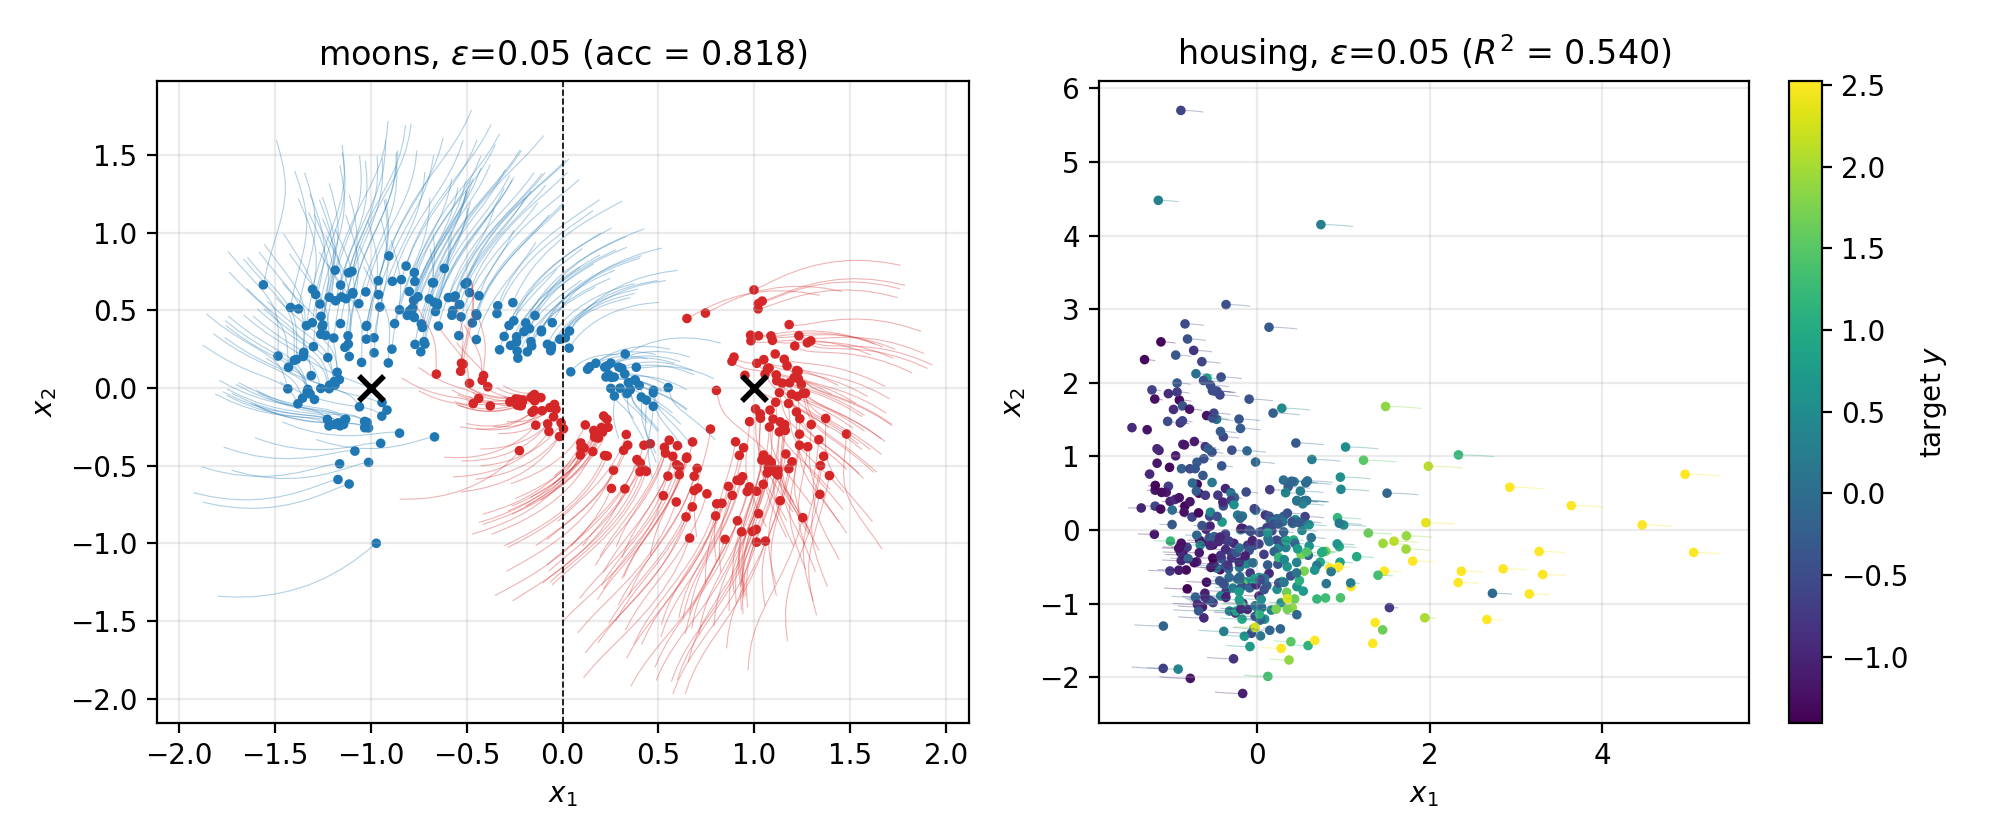
\includegraphics[width=\linewidth]{optimum_trajectories_asym_eps0.05.png}
\caption{Trajectories $t\mapsto X_i(t)$ under the optimal mean field
$\bar b(x,\nu^*_t)$ at $\eps=0.05$ (asymmetric grid).  Left: \emph{moons},
colored by class, filled dot $=X_i(T)$, crosses $=$ anchors $(\pm1,0)$.
Right: \emph{housing}, colored by the target.}
\label{fig:trajectories}
\end{figure}

Figure~\ref{fig:marginals} shows the one-dimensional marginals of $\nu^*_t$
against the prior.  Two structural features are visible.  First, the
marginals are symmetric: the Gibbs formula makes $\nu^*_t$ exactly
invariant under $a\mapsto-a$, so $\E_{\nu^*_t}[a]=0$
(Appendix~\ref{app:symmetry}); this reflects the mirror redundancy of
weight space ($b(x,-a)=b(x,a)$), not a cancellation of the field, and the
activity of the control shows in the even moments.  Second, the control is
sparse in the axes.  On \emph{moons} the output amplitudes $a_0^{(1)},
a_0^{(2)}$ and the input weight $a_1^{(2)}$ leave the prior, widening or
becoming bimodal; the bias $a_2$ concentrates at zero, more sharply than
the prior, and $a_1^{(1)}$ departs from the prior only in the first
layers.  On
\emph{housing} the activation is much weaker and concentrated on
$a_0^{(1)}$ and $a_1^{(2)}$, consistent with a nearly linear regression.
This diagnosis is what motivated the asymmetric grid of
Section~\ref{sec:method-solver} (more nodes on the active axes).

\begin{figure}[ht]
\centering
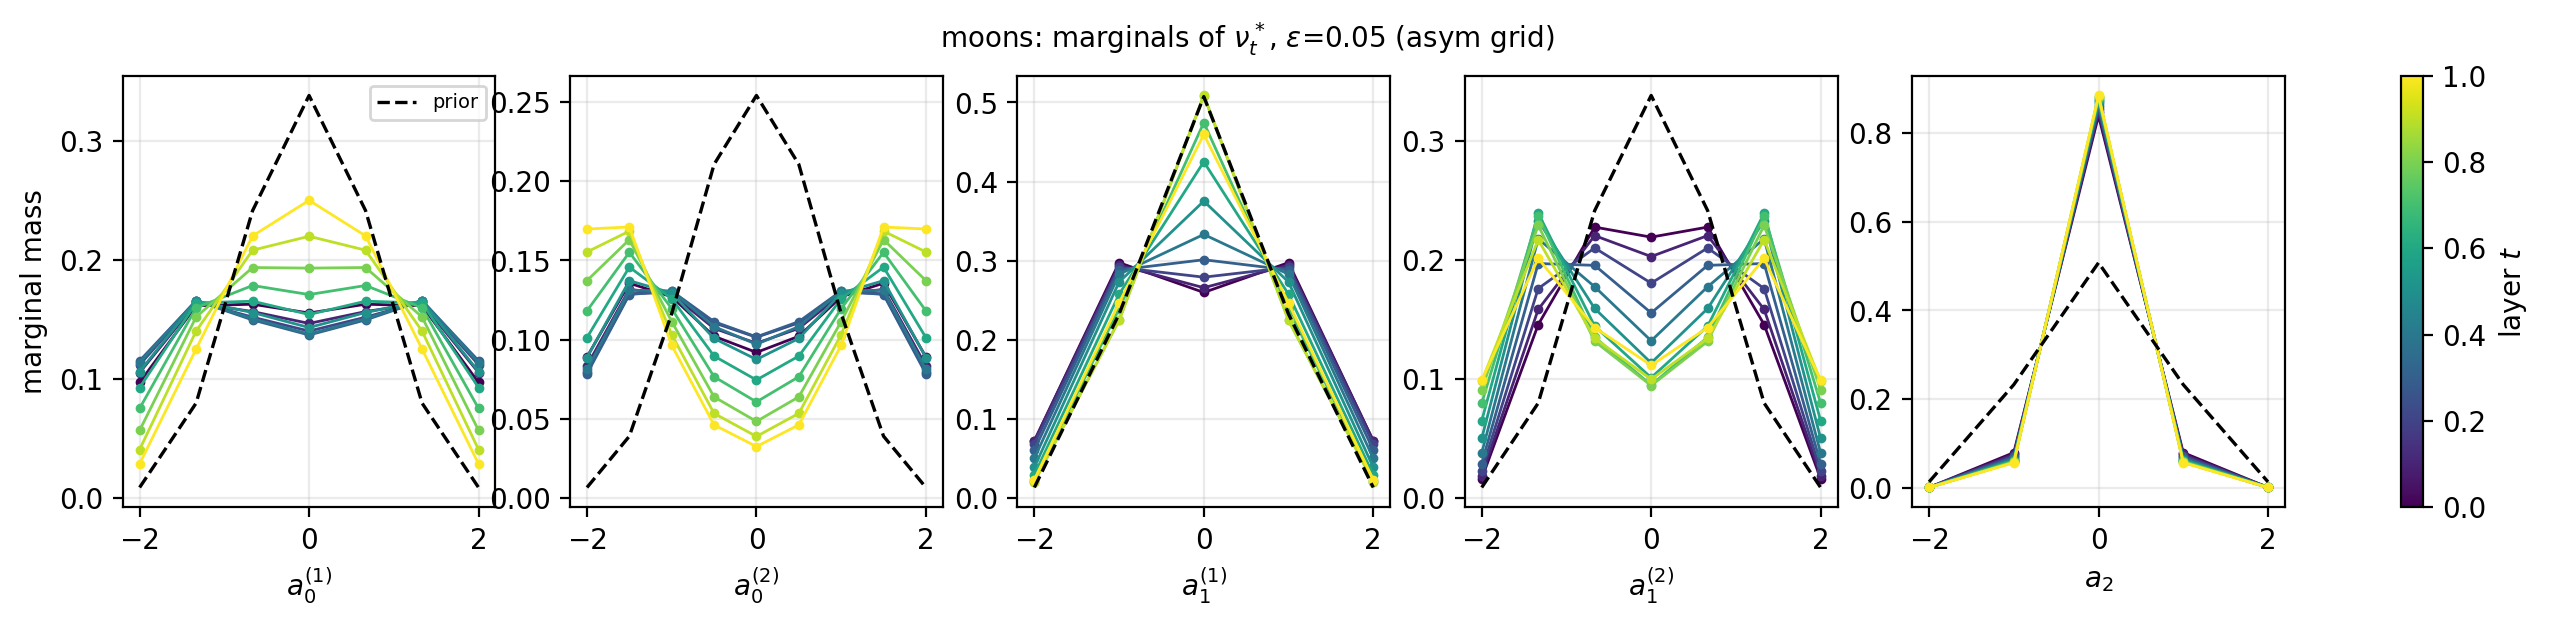
\includegraphics[width=\linewidth]{optimum_marginals_moons_asym_eps0.05.png}\\[2pt]
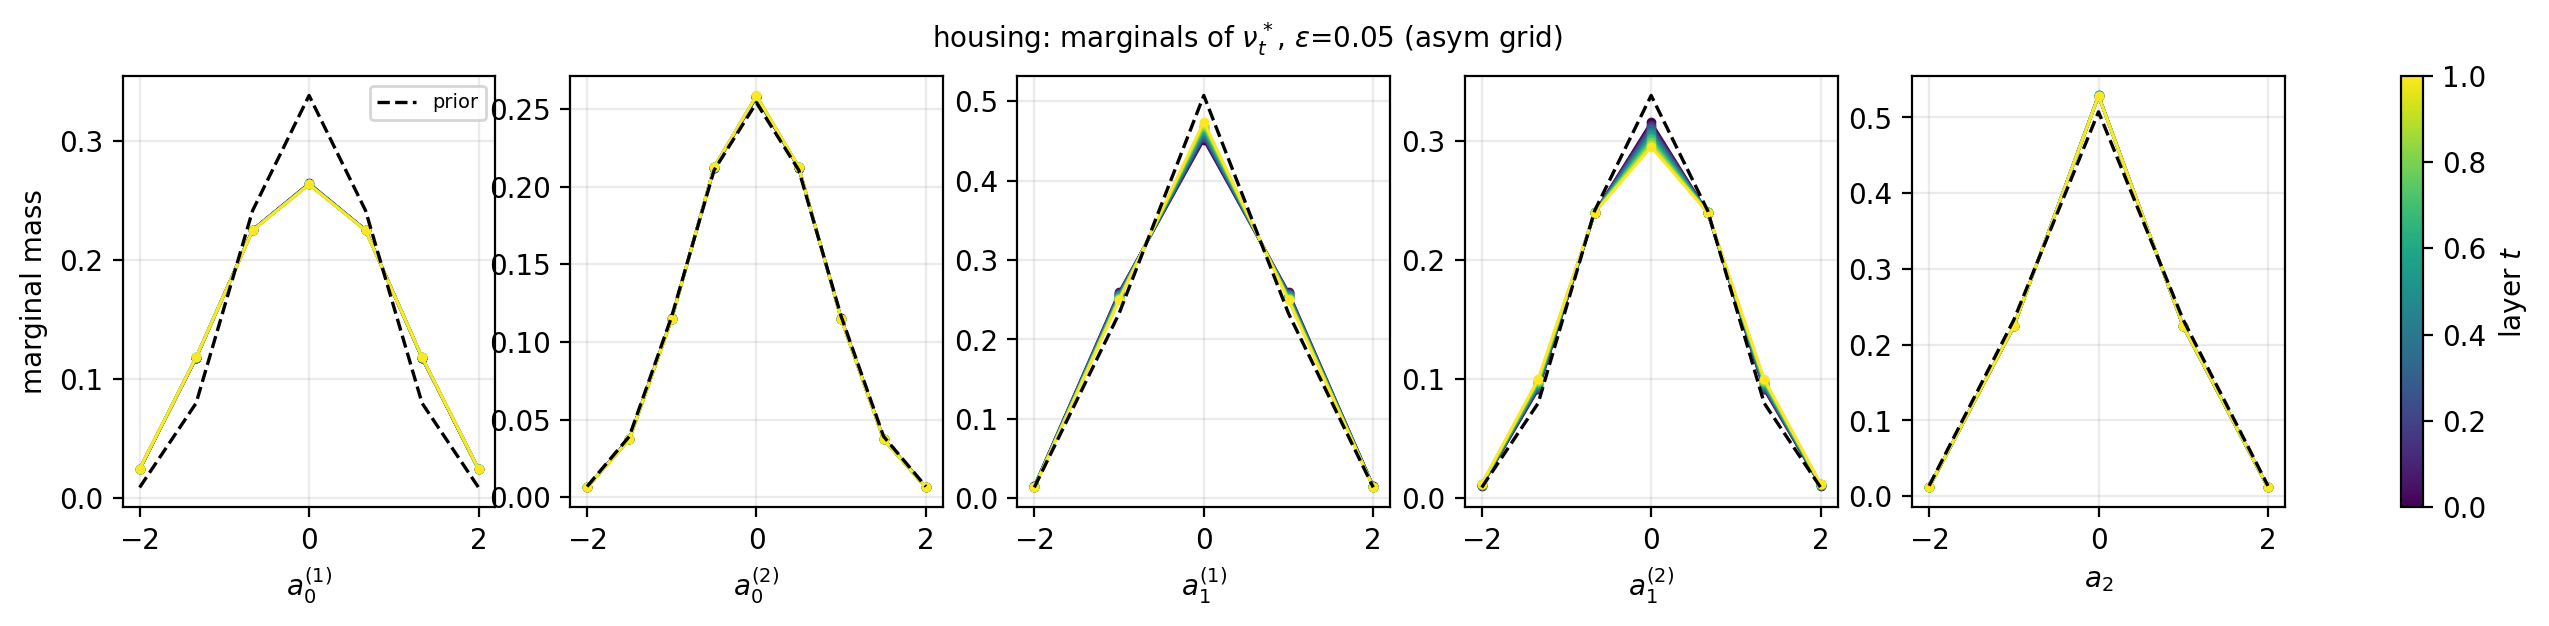
\includegraphics[width=\linewidth]{optimum_marginals_housing_asym_eps0.05.png}
\caption{One-dimensional marginals of $\nu^*_t$ at $\eps=0.05$ (color $=$
layer time $t$, dashed $=$ prior $\nu^\infty$) on the asymmetric grid.
Top: \emph{moons}.  Bottom: \emph{housing}.}
\label{fig:marginals}
\end{figure}

\subsubsection*{Concentration of the optimal control as $\eps$ decreases}
Ranking the grid nodes (``neurons'') by their time-averaged mass
$\bar w_l=\frac1{K+1}\sum_k\nu^*_{t_k}(a_l)$, Table~\ref{tab:concentration}
measures how much of the grid the optimal control actually uses: the
effective support $N_{\mathrm{eff}}=\exp(H(\bar w))$, the number $n_{50\%}$
of nodes carrying half the mass, and the overlap of the ten heaviest nodes
between the first and the last layer.  The two benchmarks behave
differently.  On \emph{moons} the mass concentrates as $\eps$ decreases
($N_{\mathrm{eff}}$ falls from $290$ nodes at $\eps=0.5$ to $145$ at
$\eps=0.05$ and $81$, $2.6\%$ of the grid, at $\eps=0.02$)
and the ranking becomes layer-dependent (only $4$ of the top-$10$ nodes at
$t=0$ remain at $t=T$ for $\eps=0.05$): the optimal network uses different
neurons at different depths.  The dominant pairs are high-gain directional
detectors: zero bias, input weights aligned with axes or diagonals, large
output amplitudes.  On \emph{housing} the concentration is essentially
insensitive to $\eps$ ($N_{\mathrm{eff}}$ stays between $284$ and $295$ down
to $\eps=0.02$) and the ranking is largely stable in depth ($7$--$9$ of the
top-$10$ nodes persist from $t=0$ to $t=T$).  This
concentration of $\nu^*_\eps$ is the mechanism invoked in
Section~\ref{sec:heuristic} to interpret the degeneration of the PL constant.

\begin{table}[ht]
\centering\small
\begin{tabular}{l r rrrc}
\toprule
benchmark & $\eps$ & mass of top-$1\%$ & $N_{\mathrm{eff}}$ & $n_{50\%}$ &
top-$10$ overlap $t=0$ vs $t=T$\\
\midrule
\emph{moons}   & 0.5  & 0.33 & 290 & 60 & 7.5/10\\
\emph{moons}   & 0.1  & 0.48 & 202 & 35 & 6.0/10\\
\emph{moons}   & 0.05 & 0.55 & 145 & 26 & 4.0/10\\
\emph{moons}   & 0.02$^\dagger$ & 0.69 & 81 & 17 & 4.0/10\\
\emph{housing} & 0.5  & 0.31 & 295 & 62 & 9.1/10\\
\emph{housing} & 0.1  & 0.32 & 293 & 61 & 7.5/10\\
\emph{housing} & 0.05 & 0.33 & 289 & 61 & 7.3/10\\
\emph{housing} & 0.02$^\dagger$ & 0.33 & 284 & 61 & 7.0/10\\
\bottomrule
\end{tabular}
\vskip 2pt
\caption{Concentration of $\bnu^*_\eps$ on the pilot grid ($M=3125$).
$N_{\mathrm{eff}}=\exp(\text{Shannon entropy of }\bar w)$.  The
$a\leftrightarrow-a$ symmetry makes node weights come in exactly equal
pairs (and, at large $\eps$, larger groups), so the top-$10$ overlap is the
expected overlap when nodes tied at the cut-off are chosen at random.
$^\dagger$Flow-refined endpoint (Section~\ref{sec:e2}(c)).}
\label{tab:concentration}
\end{table}

% ============================================================================
\section{Stability and uniqueness (Meta-Theorem 1.3)}
\label{sec:stability}

\subsection{Uniqueness: independence from the initialization}
\label{sec:uniform}
The solver starts from the prior and follows the continuation, which could
in principle select one critical point among several.  We remove both
ingredients: we start the iteration from the \emph{uniform} measure on the
grid, $\nu^{(0)}_t\equiv1/M$, far from the fixed point
($\TV(1/M,\nu^*)\approx0.9$), and run it \emph{directly} at each $\eps$,
without continuation.  All six runs (Table~\ref{tab:uniform}) converge in
$35$--$45$ iterations to the same fixed point as the continuation, at
distance of the order of the effective tolerance $\mathrm{tol}/\omega$, with
exactly zero symmetry error.  At these data and for $\eps\ge0.05$, the
critical point found is therefore not an artifact of the initialization or
of the continuation path.  This is consistent with the uniqueness part of
Meta-Theorem~1.3; the continuation is needed only to approach the regime
$\eps<0.05$.

\begin{table}[ht]
\centering\small
\begin{tabular}{l r rc c c}
\toprule
benchmark & $\eps$ & iters & conv & $J_{\mathrm{unif}}$ / $J_{\mathrm{cont}}$ &
$\TV(\nu_{\mathrm{unif}},\nu_{\mathrm{cont}})$\\
\midrule
\emph{moons}   & 0.5  & 35 & yes & 0.83385 / 0.83356 & $4.6\cdot10^{-4}$\\
\emph{moons}   & 0.1  & 37 & yes & 0.60247 / 0.60242 & $4.0\cdot10^{-4}$\\
\emph{moons}   & 0.05 & 45 & yes & 0.47521 / 0.47520 & $1.9\cdot10^{-4}$\\
\emph{housing} & 0.5  & 35 & yes & 0.27349 / 0.27321 & $5.6\cdot10^{-4}$\\
\emph{housing} & 0.1  & 35 & yes & 0.25888 / 0.25882 & $5.4\cdot10^{-4}$\\
\emph{housing} & 0.05 & 35 & yes & 0.24880 / 0.24877 & $5.2\cdot10^{-4}$\\
\bottomrule
\end{tabular}
\vskip 2pt
\caption{Uniform initialization without continuation (pilot grid).  The TV
distance (max over layers) to the continuation fixed point is at the level
of the effective tolerance $\mathrm{tol}/\omega=5\cdot10^{-4}$.}
\label{tab:uniform}
\end{table}

\subsection{E3: strict stability along the schedule}
\label{sec:e3}
Table~\ref{tab:estimators} reports $\lambda_{\min}(\eps)$ of the projected
Hessian at $\bnu^*_\eps$ (Section~\ref{sec:method-hessian}; $103$--$308$
Hessian-vector products per value).  On \emph{moons} it decreases from
$1.23$ at $\eps=0.5$ to $4.42\cdot10^{-2}$ at $\eps=0.05$ and stays strictly
positive: the computed minimizers are stable in the sense
of~\cite{DaudinDelarue2025} across the schedule --- a quantitative version of
Meta-Theorem~1.3 at these data.  Together with E1 (every sampled
perturbation increases $J$, Section~\ref{sec:e1}) this confirms that the
fixed points are strict local minima and not saddles.  The $\lambda_{\min}$
curve is not a clean power law: its local log-log slope steepens from
$1.32$ ($\eps\in[0.2,0.5]$) to $1.71$ ($\eps\in[0.05,0.1]$), a super-linear
degeneration discussed in Section~\ref{sec:heuristic}.  On \emph{housing}
$\lambda_{\min}=1.06$, $0.236$ and $0.134$ at $\eps=0.5$, $0.1$ and $0.05$:
strictly positive as well, and degenerating more slowly, with slope $0.90$
(local slopes $0.81$ and $0.93$) and no steepening.
\pending{\emph{moons} and \emph{housing} at the flow-refined $\eps=0.02$,
and \emph{housing} at $\eps=0.2$.}

\subsection{Genericity: stability under perturbations of the data}
\label{sec:genericity}
Meta-Theorem~1.3 is a statement about \emph{sets} of initial conditions,
whereas the experiments above fix one $\gamma_0$ per benchmark.  Since $\cO$
is open, a stable minimizer should persist, with a nearby value of
$\lambda_{\min}$, under small perturbations of $\gamma_0$; since it is
dense, a randomly drawn data set should fall in $\cO$.  We probe this with
families of data sets:
\emph{moons} with five sampling seeds and noise levels
$\{0.08,0.12,0.16\}$, and \emph{housing} with five training subsamples.  For
each data set we recompute the continuation on the pilot grid down to
$\eps=0.05$, $\lambda_{\min}$ at $\eps\in\{0.1,0.05\}$, and a reduced E1
cloud ($30$ perturbations) giving $c(\eps)$ (Table~\ref{tab:genericity}).
\pending{Table~\ref{tab:genericity}: expected outcome to be confirmed ---
$\lambda_{\min}>0$ for every data set, with small spread, and the same
log-log slope of $c(\eps)$.}

\begin{table}[ht]
\centering\small
\begin{tabular}{l l cc cc}
\toprule
benchmark & data variant & $\lambda_{\min}(0.1)$ & $\lambda_{\min}(0.05)$ &
$c(0.1)$ & $c(0.05)$\\
\midrule
\emph{moons}   & seeds $0$--$4$, noise $0.12$ & \pend & \pend & \pend & \pend\\
\emph{moons}   & noise $0.08$ / $0.16$       & \pend & \pend & \pend & \pend\\
\emph{housing} & subsamples $0$--$4$          & \pend & \pend & \pend & \pend\\
\bottomrule
\end{tabular}
\vskip 2pt
\caption{Genericity probe: range (min--max) over the data variants.
\pending{not yet computed.}}
\label{tab:genericity}
\end{table}

\subsection{The Jacobi condition}
\label{sec:jacobi}
Statement (a) of Theorem~4.1 can be tested without any perturbation of the
data.  For a layer index $k_1\in\{2,4,6,8\}$ we restart the problem at
$(t_{k_1},\gamma^*_{t_{k_1}})$: the particles start at the optimal
positions $X^*_i(t_{k_1})$ and the horizon is $[t_{k_1},T]$.  We solve it from
the prior, without warm start, and compare the result with the restriction
$(\nu^*_t)_{t\ge t_{k_1}}$ of the full optimum.  The theorem predicts
(i) that the two coincide (dynamic programming plus uniqueness) and (ii)
that the restarted minimizer is stable, $\lambda_{\min}(t_{k_1})>0$.  We run
this at $\eps=0.05$ on \emph{moons}.  The trapezoidal weight of the first
slice of the restarted problem differs from its weight in the full problem;
the Gibbs fixed point does not depend on the time weights, so this affects
only the Hessian, which is that of the restarted problem with its own
quadrature.  Both predictions hold (Figure~\ref{fig:jacobi}).  The four
restarted problems converge from the prior in $37$--$42$ iterations to the
restriction of the full optimum, within $\TV=3.5$--$5.5\cdot10^{-4}$, the
level of the effective tolerance $\mathrm{tol}/\omega=5\cdot10^{-4}$.  Their
minimizers are stable, with $\lambda_{\min}(t_{k_1})=0.0434$, $0.0433$,
$0.0433$ and $0.0433$ for $t_{k_1}=0.2$, $0.4$, $0.6$ and $0.8$, against
$0.0442$ for the full problem: restarting lowers $\lambda_{\min}$ by $2\%$,
after which it hardly depends on $t_{k_1}$.

\begin{figure}[ht]
\centering
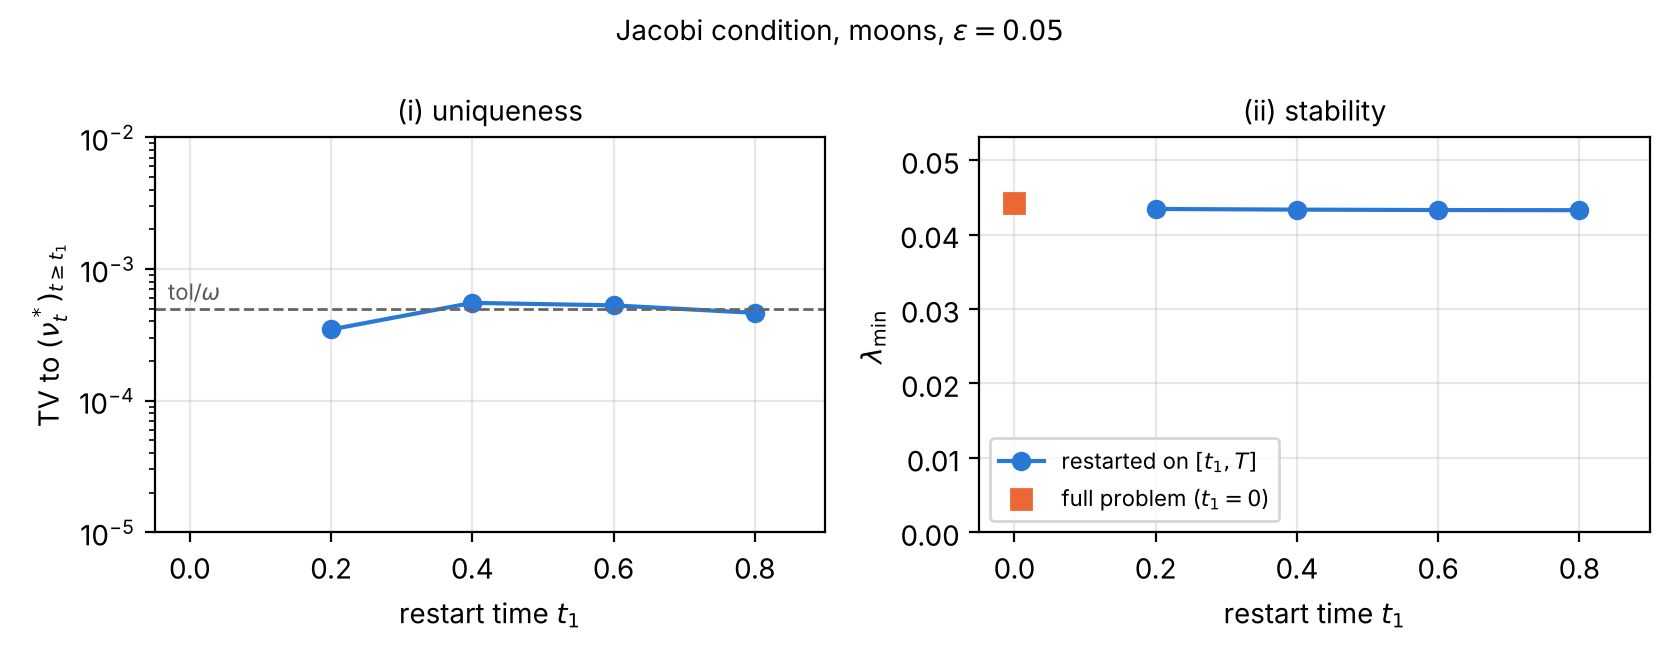
\includegraphics[width=0.85\linewidth]{jacobi_moons_eps0.05.png}
\caption{Jacobi condition (\emph{moons}, $\eps=0.05$, pilot grid).  Left:
TV distance (max over layers) between the minimizer of the problem
restarted at $(t_1,\gamma^*_{t_1})$ and the restriction of the full
optimum; dashed: effective tolerance.  Right: $\lambda_{\min}$ of the
restarted problem, and of the full problem at $t_1=0$.}
\label{fig:jacobi}
\end{figure}

% ============================================================================
\section{The PL inequality and the conjectured exponential convergence
(Meta-Theorem 1.4)}
\label{sec:pl}

\subsection{E1: the empirical PL constant \texorpdfstring{$c(\eps)$}{c(eps)}}
\label{sec:e1}
For each $\eps$ of the schedule we draw a cloud of $100$ perturbations of
$\bnu^*_\eps$ on the asymmetric grid (mixture and multiplicative-tilt
families, amplitudes $\delta\in\{0.005,0.01,0.02,0.05,0.1\}$, $10$ per
cell), evaluate $(J-J^*,\cI_h)$ for each, and set
$c(\eps)=\inf \cI_h/(J-J^*)$ over the admissible cloud
($\cI_h\ge10\,\cI_h(\bnu^*_\eps)$).  On \emph{moons}
(Table~\ref{tab:estimators}): every point of every cloud is admissible at
$\eps\ge0.05$ ($100/100$), every perturbation has $J>J^*$, all ratios are
positive --- the PL inequality holds throughout the sampled neighborhood ---
and the envelope follows a clean power law
\begin{equation}
\label{eq:c-power-law}
c(\eps)\;\propto\;\eps^{\,1.06}
\qquad(\text{log-log slope over }\eps\in[0.02,0.5];\ 0.90\text{ over }[0.05,0.5]).
\end{equation}
At $\eps=0.02$ the admissibility filter rejects the entire cloud around
the non-converged iterate ($\cI_h=8.9\cdot10^{-3}$ dominates); against the
flow-refined endpoint (Section~\ref{sec:e2}(c), $\cI_h=9\cdot10^{-11}$)
instead, $99/100$ points are admissible and $c(0.02)=0.159$, extending the
measured range to $1.4$ decades, with local slopes $0.95,0.86,0.86,1.62$:
essentially linear, steepening at the smallest $\eps$.  The clouds probe the
neighborhood in the exact sense of~\eqref{eq:PL-rigorous}: the integrated
relative entropy $\lambda^2$ ranges over $[1.2\cdot10^{-5},\,0.58]$ across
the admissible clouds, so $c(\eps)$ estimates the constant of Theorem~5.1
for entropy-radii up to $r^2\approx0.6$ at these data.  Being an infimum
over \emph{sampled} directions, $c(\eps)$ is an upper bound for the true
local constant.  On \emph{housing} the picture is the same and cleaner.
Every cloud is fully admissible ($100/100$, also at $\eps=0.02$ against the
flow-refined endpoint, where $\cI_h(\bnu^*)=1.2\cdot10^{-17}$), every
perturbation has $J>J^*$, and $c(\eps)=5.46$, $2.19$, $1.10$ and $0.227$ at
$\eps=0.5$, $0.2$, $0.1$ and $0.02$ lie on a straight line of slope $0.99$,
with local slopes between $0.98$ and $1.00$: the degeneration is linear,
with no steepening at small $\eps$ (Figure~\ref{fig:e1}).
\pending{\emph{housing} cloud at $\eps=0.05$.}

\begin{figure}[ht]
\centering
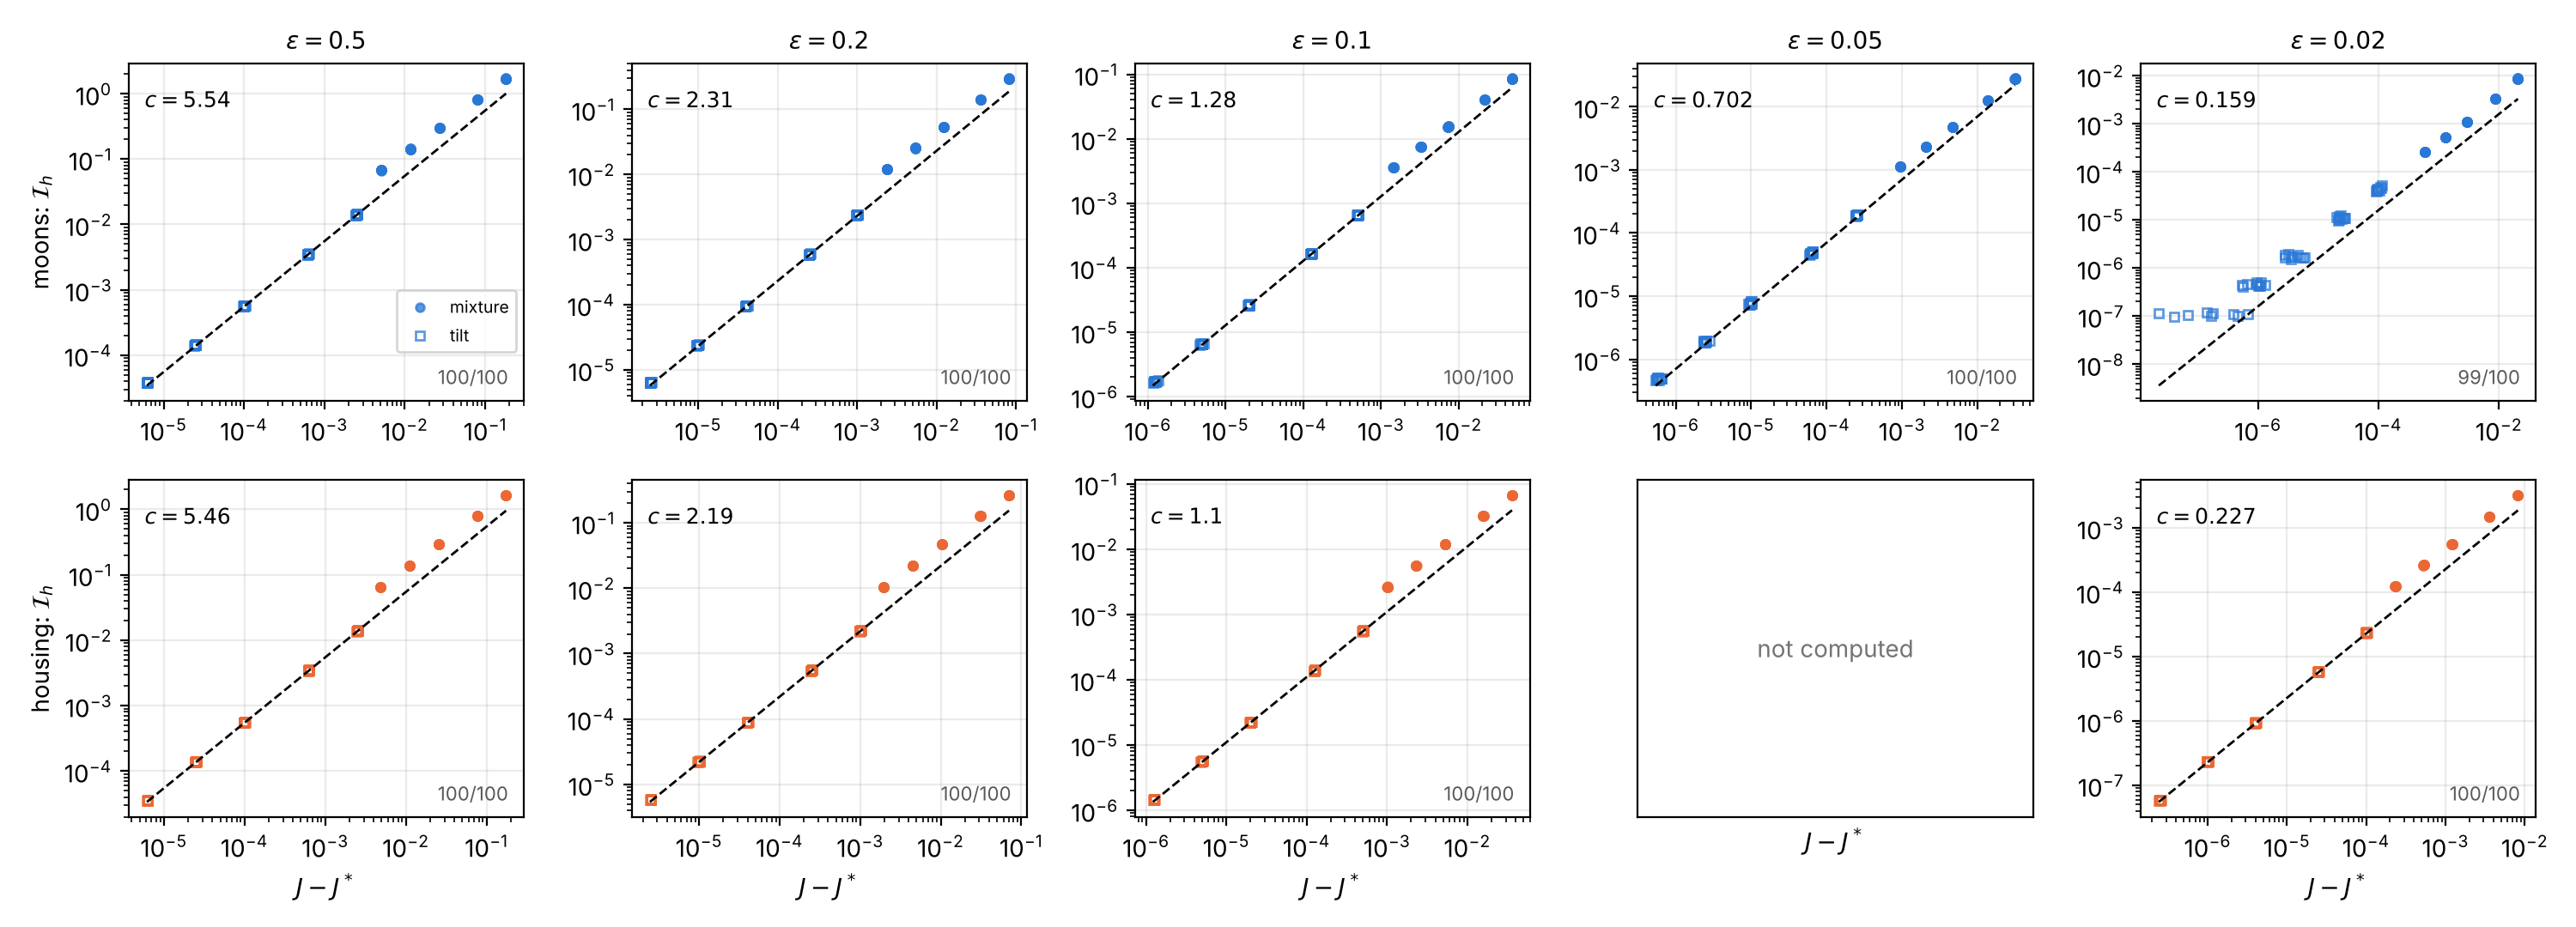
\includegraphics[width=\linewidth]{e1_scatter_asym.png}\\[2pt]
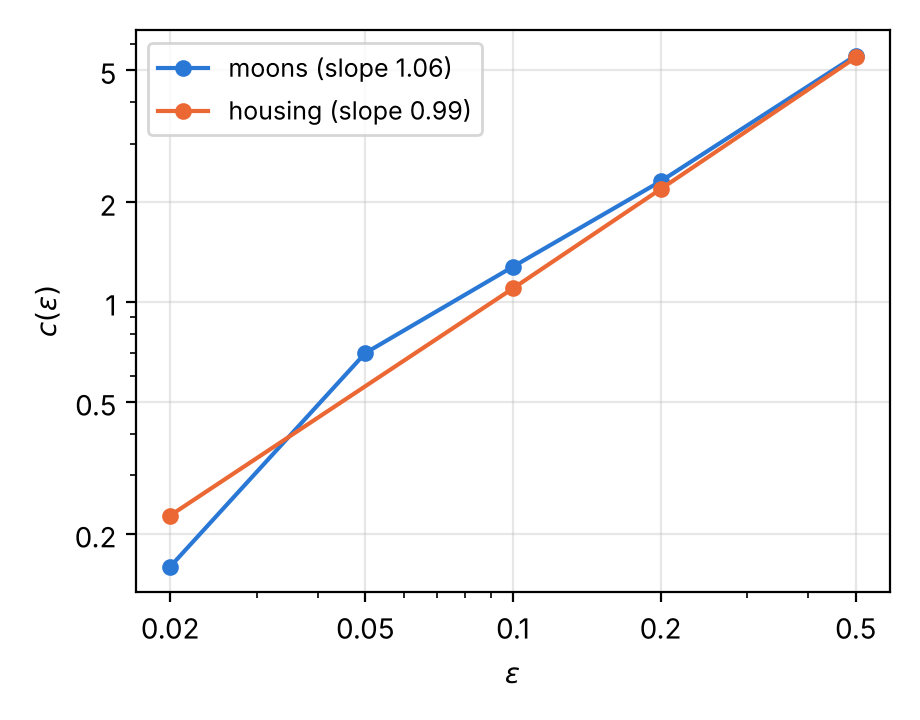
\includegraphics[width=0.5\linewidth]{e1_c_vs_eps_asym.png}
\caption{E1 (asymmetric grid).  Top: $\cI_h$ vs $J-J^*$ for the $100$-point
perturbation clouds at each $\eps$ (filled: mixtures, open: tilts; bottom
right: admissible points), with the envelope $c(\eps)=\inf\cI_h/(J-J^*)$
(dashed).  At $\eps=0.02$ the reference is the flow-refined endpoint.
Bottom: $c(\eps)$ in log-log with the least-squares slopes.}
\label{fig:e1}
\end{figure}

\subsection{E2: exponential convergence of the descent}
\label{sec:e2}
Descents are initialized at controlled TV distances from $\bnu^*$
($\delta\in\{0.02,0.05,0.1\}$, seeds $0,1,2$; $600$ steps, $\Psi$ refresh
$m=5$, pilot grid) and the slope of $\log(J(\bnu^s)-J^*)$ on the decaying
stretch (between $30\times$ and $1/3$ of the initial gap above the
tolerance floor) gives $\hat c(\eps)$.  Three observations on \emph{moons}:

\emph{(a) The conjectured exponential convergence holds.}  Every descent at
$\eps\ge0.05$ decays exponentially over $\ge4$ decades before flooring at
the solver-tolerance level $\sim(\mathrm{diffTV}/\omega)^2$ --- e.g.\ at
$\eps=0.05$ the gap falls from $1.6\cdot10^{-2}$ to $4\cdot10^{-7}$ ---, and
the floor itself confirms that the flow equilibrates at $\bnu^*$ within the
solver tolerance.  The decay is at least exponential but not a single
exponential: within every fit window the first half decays $1.3$--$1.8$
times faster than the second, as expected when the faster directions die
out first and the slowest one takes over.  The local rate stays bounded
away from zero down to the floor, which is what the PL inequality
asserts.

\emph{(b) The rate is a property of the minimizer, not of the initial
direction.}  At fixed amplitude the three seeds give the same rate to
better than $1\%$ in $10$ of the $15$ $(\eps,\delta)$ cells, and to $11\%$
in the worst (e.g.\ $\eps=0.1$, $\delta=0.1$: $\hat c=0.5994,0.5996,0.6009$);
this insensitivity to the initial direction is the PL phenomenon.  The
amplitude does matter: at every $\eps$ the rate at $\delta=0.02$ exceeds
the rate at $\delta=0.1$ by a factor $1.2$--$1.8$.  This is the transient
of (a), not a distance effect: a descent started farther away spends more
of its fit window in the regime governed by the slowest direction, so its
fitted rate is lower.  A PL constant that weakens away from $\bnu^*$ would
instead make the decay accelerate as the gap closes, the opposite of what
we see.  The medians follow
\begin{equation}
\hat c(\eps)\;\propto\;\eps^{\,1.20}\quad(\eps\in[0.02,0.5]),
\qquad
\hat c/c\in[0.47,0.74],
\end{equation}
and the exponent hardly depends on the amplitude ($1.17$, $1.20$ and $1.26$
for $\delta=0.02$, $0.05$ and $0.1$ separately).  The ratio $\hat c/c$
decreases from $0.74$ at $\eps=0.5$ to $0.47$ at $\eps=0.05$ ($0.50$ at
$\eps=0.02$).  That it is below one is expected: the cloud envelope of E1
over-estimates the true constant, whereas the descent automatically finds
the slowest direction.  At the recovered endpoint $\eps=0.02$ the amplitude
factor ($\hat c=0.095$ at $\delta=0.02$ vs $0.063$ at $\delta=0.1$, i.e.\
$1.5$) is within the range seen at larger $\eps$, so E2 gives no sign that
the PL neighborhood shrinks with $\eps$; E4 addresses that question
directly.

\emph{(c) The non-converged endpoint undershoots --- and the flow repairs
it.}  At $\eps=0.02$ every descent drives $J$ \emph{below}
$J(\bnu_{\mathrm{Picard}})$ immediately: with $\mathrm{diffTV}/\omega=0.55$
the last iterate of the fixed-point iteration is not the minimizer.  Turning
the observation into a tool, we integrate the flow \emph{from} that iterate
until $\cI_h$ plateaus (the \emph{flow-refined endpoint}).  On the pilot
grid the refinement moves the control by $\TV=0.55$ --- exactly the
calibrated defect ---, lowers the cost from $0.3421$ to $0.3192$, drives
$\cI_h$ from $9\cdot10^{-3}$ to $10^{-8}$, and its fixed-point residual
after one \emph{undamped} Gibbs update is
$\TV(\nu_{\mathrm{Gibbs}},\nu)=2.6\cdot10^{-7}$: the refined control
\emph{is} the Gibbs fixed point, reached where the fixed-point iteration has
lost contractivity (Section~\ref{sec:method-solver}).  Test accuracy is
essentially unchanged ($0.930$ vs $0.935$).  This recovers the $\eps=0.02$
endpoint for E1/E2 and suggests \emph{Picard-then-flow} as the standard
pipeline at small $\eps$.  Figure~\ref{fig:e2} shows the decay curves.

\emph{(d) Convergence of the trajectory.}  Beyond the cost, the authors
suggest that the control itself should converge exponentially
(cf.~\cite{monmarche2024local}).  Along the same descents we record the
integrated relative entropy $\int\cE(\nu^s_t|\nu^*_t)\dd t$, the very
distance in which Theorem~5.1 measures the PL neighborhood.  At
$\eps\in\{0.5,0.2\}$, where it was recorded on both benchmarks, it decays
exponentially at the same rate as the cost: the median fitted rates are
$4.13$ and $1.54$ on \emph{moons} (against $\hat c=4.12$ and $1.41$) and
$3.97$ and $1.61$ on \emph{housing} (against $3.98$ and $1.55$), ratios
between $1.00$ and $1.09$.  Since $J-J^*$ and the integrated entropy are
both quadratic in $\bnu-\bnu^*$ near the minimizer, equal rates are what
exponential convergence of the control itself predicts.
\pending{the entropy decay at $\eps\le0.1$.}

On \emph{housing} the descents at $\eps=0.5$ and $0.2$ behave as on
\emph{moons}: median rates $\hat c=3.98$ and $1.55$, seeds agreeing to
better than $0.1\%$ in $5$ of the $6$ $(\eps,\delta)$ cells, and the same
amplitude factor ($1.26$ and $1.19$).
\pending{\emph{housing} descents at $\eps\in\{0.1,0.05\}$ and at the
flow-refined $\eps=0.02$ endpoint.}

\begin{figure}[ht]
\centering
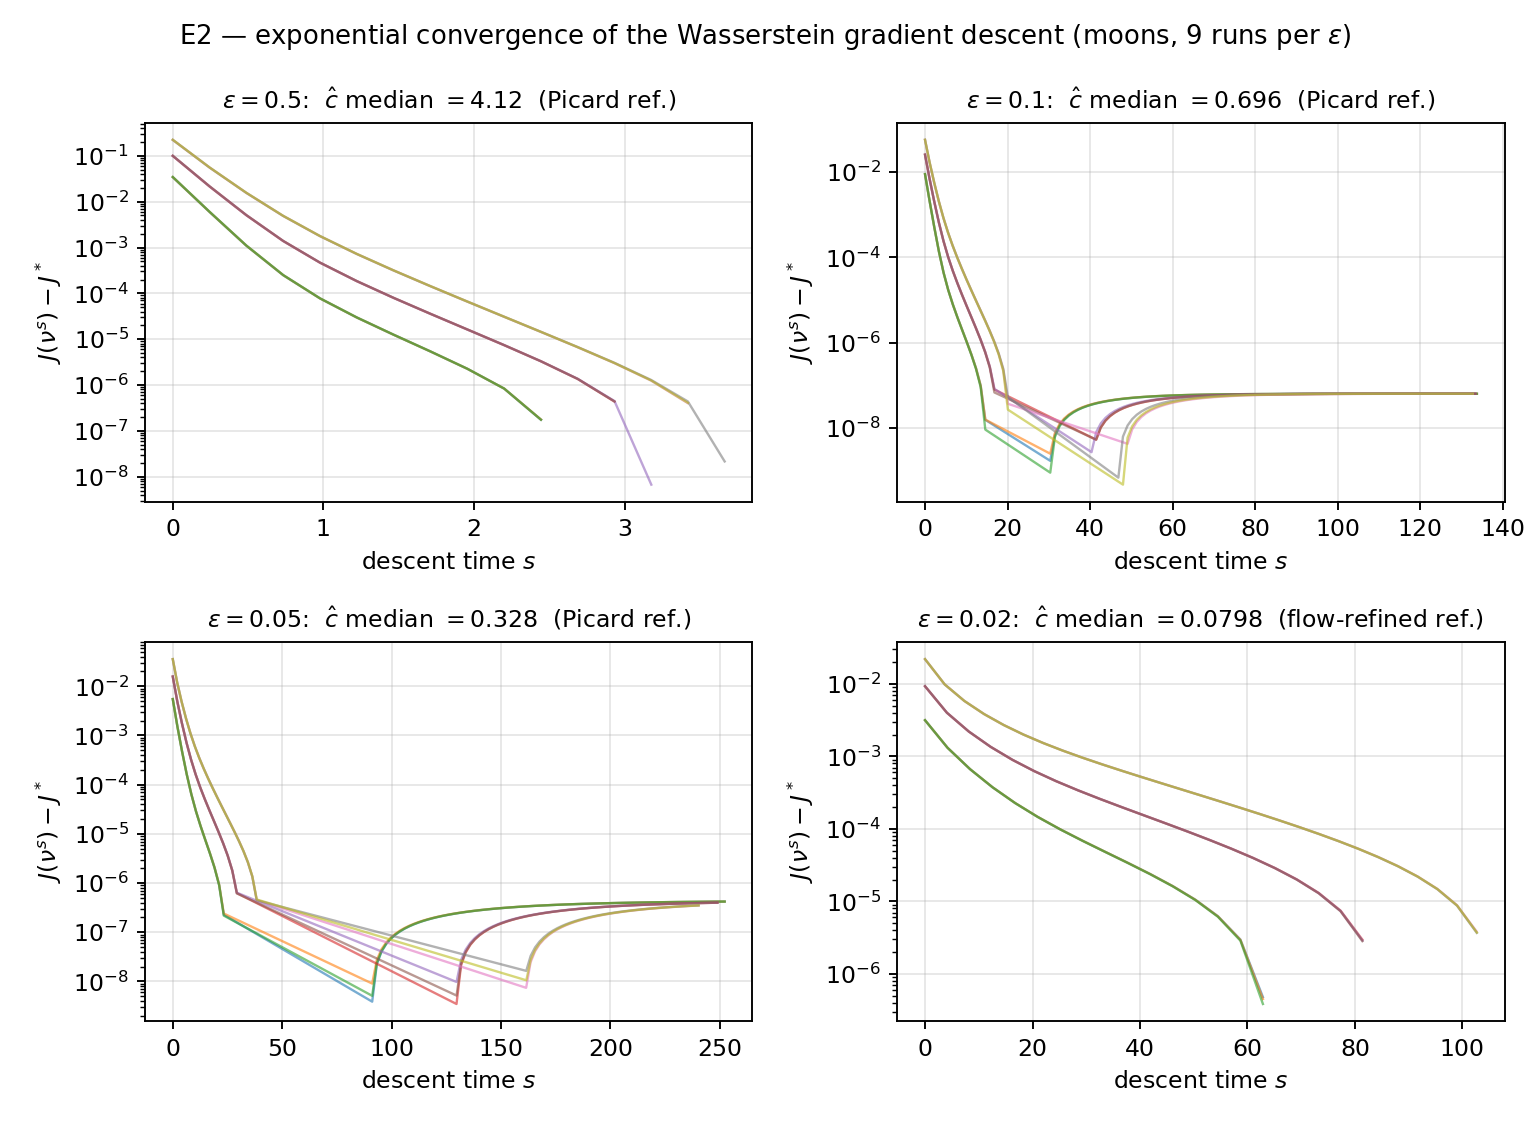
\includegraphics[width=\linewidth]{e2_panel_moons.png}
\caption{E2 (\emph{moons}, pilot grid): $J(\bnu^s)-J^*$ for the nine
(amplitude, seed) descents at four values of $\eps$.  The decay is
exponential over $\ge4$ decades down to the solver-tolerance floor; at
$\eps=0.02$ the reference is the flow-refined endpoint.}
\label{fig:e2}
\end{figure}

\subsection{E4: radius of the PL neighborhood}
\label{sec:e4}
We sweep mixture perturbations of increasing amplitude
$\delta\in[0.02,0.9]$ ($6$ per amplitude, \emph{moons}, $\eps=0.05$,
asymmetric grid) and monitor the worst ratio $\cI_h/(J-J^*)$ against the
small-amplitude envelope $c(0.05)=0.70$ of E1.  No boundary is visible:
the minimal ratio stays in $[0.89,\,1.08]$ across the whole sweep --- it
dips mildly around $\delta\approx0.1$--$0.2$ and \emph{increases} again
for $\delta\ge0.5$ --- and not a single perturbation falls below
$c(0.05)$.  Within this perturbation family the local PL inequality is, in
practice, global at moderate $\eps$: the entropy radius $r$ exceeds
everything we can reach with $\TV\le0.9$ ($\lambda^2$ up to $7.2$).  Nor
does E2 show a finite neighborhood: the amplitude dependence of $\hat c$ is
present at every $\eps$, is no stronger at $\eps=0.02$, and goes the wrong
way for one (Section~\ref{sec:e2}(b)).  Whether the radius shrinks with
$\eps$ is therefore open.  The caveat is plain: one perturbation family,
one $\eps$.

\subsection{The degeneration picture}
\label{sec:degeneration}

\begin{table}[ht]
\centering\small
\begin{tabular}{l rrr @{\qquad} rrr}
\toprule
& \multicolumn{3}{c}{\emph{moons}} & \multicolumn{3}{c}{\emph{housing}}\\
$\eps$ & $c$ (E1) & $\hat c$ (E2) & $\lambda_{\min}$ (E3)
       & $c$ (E1) & $\hat c$ (E2) & $\lambda_{\min}$ (E3)\\
\midrule
0.5  & 5.54 & 4.12 & 1.233  & 5.46 & 3.98 & 1.062\\
0.2  & 2.31 & 1.41 & 0.368  & 2.19 & 1.55 & \pend\\
0.1  & 1.28 & 0.70 & 0.144  & 1.10 & \pend & 0.236\\
0.05 & 0.70 & 0.33 & 0.0442 & \pend & \pend & 0.134\\
0.02$^\dagger$ & 0.159 & 0.080 & \pend & 0.227 & \pend & \pend\\
\midrule
log-log slope & 1.06 & 1.20 & 1.43 & 0.99 & \pend & 0.90\\
\bottomrule
\end{tabular}
\vskip 2pt
\caption{The three estimators of the PL degeneration (E1 on the asymmetric
grid; E2, E3 on the pilot grid; $\hat c$ is the median of $9$ descents).
Slopes over the computed values.
$^\dagger$Relative to the flow-refined endpoint ($99/100$ admissible cloud
points on \emph{moons}, $100/100$ on \emph{housing}; the non-converged
iterate admits none on \emph{moons}).}
\label{tab:estimators}
\end{table}

The two completed estimators on \emph{moons} give power laws with exponents
close to one: the PL constant of~\cite{DaudinDelarue2025} degenerates
\emph{essentially linearly in $\eps$}, which quantifies the non-uniformity
in $\eps$ that the authors flag as an open direction.
Figure~\ref{fig:star} superposes the three estimators in log-log.
$\lambda_{\min}(\eps)$ --- which lives in a different (Euclidean,
grid-dependent) normalization and sits an order of magnitude below ---
degenerates faster on \emph{moons} (slope $1.43$) and shares with $c$
and $\hat c$ the super-linear steepening at the smallest $\eps$.  On
\emph{housing} the degeneration is linear without steepening:
$c\propto\eps^{0.99}$ down to $\eps=0.02$ and $\lambda_{\min}\propto
\eps^{0.90}$.

\begin{figure}[ht]
\centering
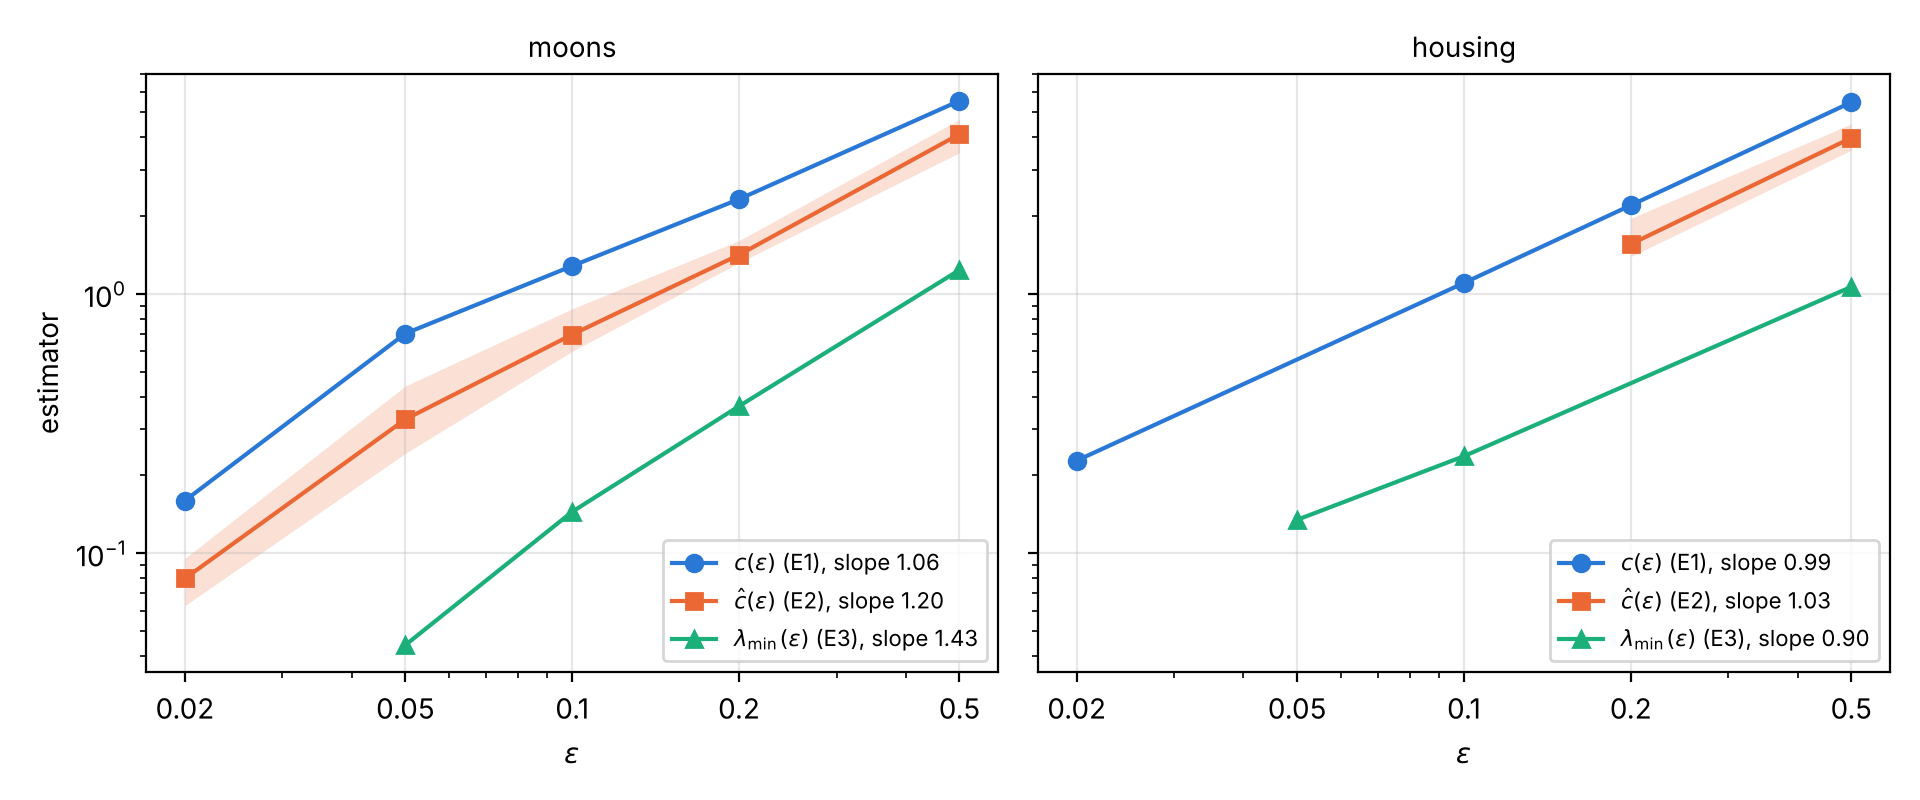
\includegraphics[width=\linewidth]{star_asym.png}
\caption{The three independent estimators of the PL degeneration in log-log,
with least-squares slopes; the band is the min--max of the nine descents of
E2.  Left: \emph{moons}.  Right: \emph{housing}.}
\label{fig:star}
\end{figure}

% ============================================================================
\section{Discussion}
\label{sec:discussion}

\subsection{Why (essentially) linear degeneration: a heuristic}
\label{sec:heuristic}
The measured exponents cluster around $1$, and a two-line expansion suggests
why this should be the leading behavior.  Write
$\nu_t=\nu^*_t(1+\varphi_t)$ for a small relative perturbation and let
$\eta=\nu-\bnu^*$.  Since the Gibbs formula cancels the integrand of
$\cI$ at $\bnu^*$,
\[
\cI(\bnu)\;\approx\;\int_{t_0}^T\!\!\int_A
\bigl|\,\eps\nabla_a\varphi_t+\delta[\nabla_a\Psi_t](\eta)\,\bigr|^2
\dd\nu^*_t\dd t,
\qquad
J-J^*\;\approx\;\tfrac12\Bigl[\eps\!\int_{t_0}^T\!\!\int_A\varphi_t^2
\dd\nu^*_t\dd t+\langle H_\Psi\eta,\eta\rangle\Bigr],
\]
where $\delta[\nabla_a\Psi](\eta)$ and $H_\Psi$ carry the terminal cost and
are $O(\eta)$ uniformly in $\eps$, while the entropic contributions carry
explicit factors $\eps^2$ (in $\cI$) and $\eps$ (in $J-J^*$).  For
directions nearly invisible to the terminal cost --- abundant, since the
data see the parameter space only through $N$ particles --- the ratio
reduces to a Rayleigh quotient,
\[
\frac{\cI}{J-J^*}\;\approx\;
2\eps\,\frac{\int\!\!\int|\nabla_a\varphi|^2\dd\nu^*\dd t}
              {\int\!\!\int\varphi^2\dd\nu^*\dd t}
\;\ge\;2\eps\,\rho(\bnu^*_\eps),
\]
with $\rho$ the (worst-slice) Poincar\'e constant of $\nu^*_\eps$.  If
$\rho(\bnu^*_\eps)=O(1)$ over the measured range, $c(\eps)\propto\eps$.  The
deviations from slope one then encode the $\eps$-dependence of the spectral
constants of $\nu^*_\eps$ itself, i.e.\ how the concentration of the Gibbs
measure (Table~\ref{tab:concentration}) competes with the vanishing
prefactor.  This is consistent with the steepening being visible on
\emph{moons}, where $\nu^*_\eps$ concentrates markedly as $\eps$ decreases,
and with the behavior on \emph{housing}, where it does not: there the
local slopes of $c(\eps)$ stay between $0.98$ and $1.00$ down to
$\eps=0.02$, as predicted for $\rho(\bnu^*_\eps)=O(1)$.  The
same expansion predicts $\lambda_{\min}(\eps)\propto\eps$ for the entropic
block of the Hessian, up to the grid-dependent Euclidean normalization;
only the \emph{slope} of $\lambda_{\min}(\eps)$ is comparable across
estimators.  In the terminology of~\cite{DaudinDelarue2025}, the local PL
constant is not merely non-uniform but vanishes at an essentially linear
rate, consistent with the entropic term being the sole source of local
convexity; in the unregularized limit the landscape changes nature
altogether~\cite{lu2020mean}.

\subsection{Methodological recommendations}
(i) Report $\mathrm{diffTV}/\omega$, not $\mathrm{diffTV}$: it is the
distance all downstream tolerances inherit.  (ii) When a damped fixed-point
iteration stalls, check for a period-2 cycle before blaming the
continuation step.  (iii) Discretize first variations compatibly, so that
the discrete minimizer is an exact critical point.  (iv) Use
exponential-fitting fluxes for measure-space gradient flows, so that the
discrete equilibrium is the discrete Gibbs measure; the flow is then also a
robust solver where the fixed-point iteration fails.  (v) Split
Hessian-vector products into the exact entropic diagonal plus differences
of the smooth part, and remove the projected null space before computing
$\lambda_{\min}$.

\subsection{Limitations and outlook}
The solver meshes $A$, so everything lives in low dimension ($d'=5$);
generalizing beyond tensor grids (adaptive grids concentrated on the
effective support of Table~\ref{tab:concentration}, sparse grids, particle
discretizations) is open.  The clean measurements span $1.4$ decades of
$\eps$, bounded below by the loss of contractivity of the fixed-point
iteration; Newton-type solvers or $\eps$-dependent damping would extend the
range, subject to grid resolution.  Our genericity probe samples data sets
near two benchmarks and cannot exhibit the complement of $\cO$; locating
non-generic data (e.g.\ symmetric data sets where several minimizers could
coexist) is a natural next step.  Finally, $\hat c$ is measured through one
discretization of the Wasserstein flow; its agreement in slope with the
discretization-independent ratio estimator $c(\eps)$ is our main evidence
that the measured degeneration is not a numerical artifact.  Two questions
raised in~\cite{DaudinDelarue2025} remain for future work: the convergence
of $J^*$ and $\bnu^*$ as the number $N$ of data points grows (with rates
expected to improve when $\gamma_0\in\cO$), and the approximation of
$\bnu^*$ by networks with finitely many neurons.

\subsection*{Acknowledgments}
The author thanks Rafael Orive Illera for supervising this work, which
was carried out at ICMAT within the JAE Intro training plan ``Neural ODEs y
Machine Learning'' (JAEINT25\_EX\_1604).  Funding: JAE Intro 2025
fellowship of the Spanish National Research Council (CSIC), reference
JAEINT\_25\_03361.

% ============================================================================
\appendix

\section{Characteristics and the Jacobian cocycle}
\label{app:cocycle}
With the mean field frozen, the characteristics of the backward transport
equation $-\partial_tu_t-\bar b(x,\nu_t)\cdot\nabla_xu_t=0$, $u_T=L$, are
the forward particle trajectories $\dot X_t=\bar b(X_t,\nu_t)$, and
$\frac{d}{dt}u_t(X_t,y)=\partial_tu_t+\nabla_xu_t\cdot\bar b=0$.  Hence
$u_t(X_t(x_0),y)=L(X_T(x_0),y)$ for every $x_0$.  Differentiating in $x_0$
with $\Phi_s=\partial X_s/\partial x_0$ gives
$\Phi_t^\top\nabla_xu_t(X_t,y)=\Phi_T^\top\nabla_xL(X_T,y)$, and since the
flow is a diffeomorphism, $\nabla_xu_t(X_t,y)=[\Phi_T\Phi_t^{-1}]^\top
\nabla_xL(X_T,y)$ --- formula~\eqref{eq:cocycle}.  The Jacobians solve
$\dot\Phi=\partial_x\bar b(X,\nu_t)\Phi$, $\Phi(0)=I$, and are integrated
by RK4 jointly with the particles.  Meshing $\R^{d_1}$ for the backward PDE
would scale exponentially in $d_1$; the cocycle costs $O(Nd_1^3)$ per slice
and needs no spatial mesh.

\section{The exact \texorpdfstring{$a\leftrightarrow-a$}{a <-> -a} symmetry}
\label{app:symmetry}

\begin{prop}[$a\leftrightarrow-a$ invariance of the optimal control]
\label{prop:symmetry}
With $\sigma=\Tanh$ (odd) and $\ell$ even, any control given by the Gibbs
formula~\eqref{eq:gibbs} satisfies, for every $t$,
\[
\nu^*_t(-a)=\nu^*_t(a)\quad\forall a\in A,
\qquad\text{hence}\qquad
\E_{\nu^*_t}[a]=0 .
\]
The invariance is structural: it depends only on the parities of
$b(x,\cdot)$ and $\ell$, not on $\gamma_0$, $L$ or $\eps$.
\end{prop}

\begin{proof}
Write the Gibbs exponent as $-\ell(a)-\Psi_t(a)/\eps$ with $\Psi_t$ as
in~\eqref{eq:gibbs}.  (i) $\ell(-a)=\ell(a)$ since $\ell$ depends on $|a|$.
(ii) Negating the three blocks of $a=(a_0,a_1,a_2)$ and using that $\Tanh$
is odd,
\[
b(x,-a)=\Tanh(-a_1\!\cdot\!x-a_2)(-a_0)=\Tanh(a_1\!\cdot\!x+a_2)\,a_0
=b(x,a),
\]
so $b(x,\cdot)$ is \emph{even}.  (iii) The pair $(\gamma_t,u_t)$ does not
depend on $a$, hence $\Psi_t(-a)=\Psi_t(a)$ by (ii).  The exponent is
therefore even, giving $\nu^*_t(-a)=\nu^*_t(a)$; and $a\,\nu^*_t(a)$ is odd,
so its integral over the symmetric domain vanishes.
\end{proof}

\begin{rmk}
The zero first moment reflects the mirror redundancy of weight space
($b(x,-a)=b(x,a)$: $a$ and $-a$ implement the same map and their
contributions to $\bar b$ reinforce), not a cancellation of the control.
On our odd-$m_j$ grids, which are symmetric under $a\mapsto-a$, the Gibbs
update produces exactly even node weights, so the discrete $\nu^*$ is
symmetric to machine precision (error $0.0$ bitwise along the whole
schedule, $\max_i|\E[a_i]|\lesssim6\cdot10^{-16}$), and the discrete flow
preserves it.  Any asymmetric bug in the forward pass, the cocycle or the
Gibbs update breaks this test immediately.
\end{rmk}

\section{Reproducibility}
\label{app:repro}

All code, frozen $\bnu^*$ checkpoints and experiment outputs are available
at \url{https://github.com/dantor03/mfnode-pl-verification}
\todo{tag the submission commit}.  The library is pure Python
($\ge3.10$) on \texttt{numpy}/\texttt{scipy}/\texttt{scikit-learn}; no GPU
is used.  The correctness suite (\texttt{pytest tests/}, $18$ tests,
$\approx4$\,s) covers every structural property quoted in
Section~\ref{sec:method-tests}.

\subsection*{Data}
Every random object derives from the single seed $\mathrm{SEED}=42$.
\emph{moons}: \texttt{make\_moons} with $n=400$, noise $0.12$,
standardized; labels embedded as anchors $(\pm1,0)$.
\emph{housing}: California Housing, subsample of $600$ rows
($400$ train, $200$ test, split seed $42$), features and target
standardized, restricted to the two features with largest
$|\mathrm{corr}|$ with the target on the train split (MedInc, AveOccup).
Genericity probe (Section~\ref{sec:genericity}): \emph{moons} with
sampling seeds $0$--$4$ at noise $0.12$, and seed $42$ at noise $0.08$ and
$0.16$; \emph{housing} with subsample and split seeds $0$--$4$ ($600$ rows,
$400$ train), the two features fixed to MedInc and AveOccup so that only
the sample changes.

\subsection*{Hyperparameters}
\begin{center}\small
\begin{tabular}{ll}
\toprule
horizon / slices & $T=1$, $K=10$ (trapezoidal $w_k$)\\
prior & $\ell(a)=0.05|a|^4+0.5|a|^2$\\
parameter box & $A=[-2,2]^{5}$\\
grids & pilot $m_j\equiv5$ ($M=3125$); asymmetric $m=(7,9,5,7,5)$ ($M=11025$)\\
fixed-point iteration & $\omega=0.2$, $\mathrm{tol}=10^{-4}$ on diffTV, $\mathrm{max\_iter}=200$\\
continuation & $\eps\in(0.5,0.2,0.1,0.05,0.02)$, warm starts; fine: $(0.04,0.03,0.025,0.02)$\\
Fisher & compatible (fd) assembly, $\log\nu$ floored at $-40$\\
flow & Scharfetter--Gummel, explicit Euler at $0.9\times$CFL,\\
     & $\Psi$ refreshed every $m=5$ steps, per-slice renormalization\\
Hessian & central step $h=10^{-5}$, support threshold $10^{-6}$,\\
        & LOBPCG with entropic-diagonal preconditioner, null-space penalty $\sigma=100$\\
\bottomrule
\end{tabular}
\end{center}

\subsection*{Timings}
Single laptop CPU: $\approx9$\,s (pilot) and $\approx35$\,s (asymmetric)
per fixed-point iteration; full continuations $0.5$--$5$\,h; E1 $\approx2$\,h
and E2 $1$--$2$\,h per $\eps$; E3 $0.3$--$3.6$\,h per eigenvalue; flow
refinement of the $\eps=0.02$ endpoint $1$\,h (pilot) to $7$\,h
(asymmetric).  Every $\bnu^*$ is stored as a resumable checkpoint consumed
unchanged by all experiment runners.


% ============================================================================
\bibliographystyle{abbrv}
\bibliography{references}

\end{document}
